\documentclass[t,handout]{beamer}
\usepackage[default]{sourcesanspro}
% \usepackage[default]{sourcecodepro}
% \usepackage[default]{sourceserifpro}
\usepackage[utf8]{inputenc}
\usepackage[english]{babel}
\usepackage{listings}
\lstset{ %
  basicstyle=\ttfamily\color{black}\tiny,
  breaklines=true,
  columns=fullflexible,
  frame=single,
  keepspaces=true,
  tabsize=2
}

\definecolor{darkblue}{rgb}{0,0,.5}
\hypersetup{pdftex=true, colorlinks=true, breaklinks=true, linkcolor=darkblue, menucolor=darkblue, pagecolor=darkblue, urlcolor=darkblue}

\title{Timewarrior -- Where did my time go?}
\subtitle{Introduction}
\author[Deimeke, Dirk]{Dirk Deimeke}
\institute[Taskwarrior academy]{Taskwarrior academy}
\date{FrOSCon 2016}
\titlegraphic{
\includegraphics[width=3cm,height=3cm]{tw-xxl}}
\subject{Timewarrior}
\keywords{timewarrior, time, management, commandline}

\setbeamercovered{transparent}

\pgfdeclareimage[width=5mm]{tw-logo}{tw-xl}

%%%%%%%%%%%%%%%%%%%%%%%%%%%%%%%%%%%%%%%%%%%%%%%%%%%%%%%%%%%%%%%%%%%%%%%
%
% LaTeX-Template for Taskwarrior by Dominik Wagenführ
% http://www.deesaster.org/
%
% Creative Commons Attribution-ShareAlike 4.0 (CC-BY-SA 4.0)
% https://creativecommons.org/licenses/by-sa/4.0/
%
%%%%%%%%%%%%%%%%%%%%%%%%%%%%%%%%%%%%%%%%%%%%%%%%%%%%%%%%%%%%%%%%%%%%%%%

%%%%%%%%%%%%%%%%%%%%%%%%%%%
% Layout - Start
%%%%%%%%%%%%%%%%%%%%%%%%%%%

\setbeamertemplate{navigation symbols}{}

\useinnertheme{default}
\useoutertheme{infolines}
\usefonttheme{structurebold}

\newlength{\boxwidth}
\setlength{\boxwidth}{121px}
\setbeamertemplate{headline}{%
\begin{beamercolorbox}[dp=3px,ht=6px,wd=\boxwidth,center]{palette tertiary}%
\insertauthor\ (\insertinstitute)%
\end{beamercolorbox}%
\vskip-9px\hskip\boxwidth
\begin{beamercolorbox}[dp=3px,ht=6px,wd=\boxwidth,center]{palette secondary}%
\inserttitle%
\end{beamercolorbox}%
\begin{beamercolorbox}[dp=3px,ht=6px,wd=\boxwidth,right]{palette primary}%
\insertdate\hskip15px\insertframenumber\,/\,\inserttotalframenumber\hspace*{8px}
\end{beamercolorbox}%
}
\setbeamertemplate{footline}{}

%%%%%%%%%%%%%%%%%%%%%%%%%%%
% Colors - Start
%%%%%%%%%%%%%%%%%%%%%%%%%%%

\definecolor{basecolor}{gray}{0.2}
\definecolor{mittelgrau}{gray}{0.4}
\definecolor{hellgrau}{gray}{0.93}
\definecolor{gelb}{rgb}{1.0,1.0,0.75}

% infolines color
\setbeamercolor{palette primary}{fg=white,bg=mittelgrau}
\setbeamercolor{palette secondary}{fg=white,bg=basecolor}
\setbeamercolor{palette tertiary}{fg=white,bg=black}

% frame and title color
\setbeamercolor{frametitle}{fg=white,bg=basecolor}
\setbeamercolor{titlelike}{fg=white,bg=basecolor}
\setbeamerfont{frametitle}{series=\bfseries}

% TOC color
\setbeamercolor{section in toc}{fg=basecolor}

% text color
\setbeamercolor{normal text}{fg=black,bg=white}

% item color
\setbeamercolor{item}{fg=basecolor}
\setbeamercolor{itemize item}{fg=black}

% block color
\setbeamercolor{block title}{fg=black,bg=gelb}
\setbeamercolor{block body}{fg=black,bg=gelb}

% block alert color
\setbeamercolor{block title alerted}{fg=black,bg=gelb}
\setbeamercolor{block body alerted}{fg=black,bg=gelb}

% block example color
\setbeamercolor{block title example}{fg=black,bg=gelb}
\setbeamercolor{block body example}{fg=black,bg=gelb}

\setbeamertemplate{frametitle}{%
\vskip-1px%
\begin{beamercolorbox}[wd=363px,ht=20px,dp=12px]{frametitle}
\usebeamerfont{frametitle}%
\usebeamercolor{frametitle}%
\vspace*{-5px}\hspace*{10px}
\includegraphics[width=24px,height=24px]{tw-xl.png}\\
\vspace*{-20px}\hspace*{40px}\insertframetitle%
\end{beamercolorbox}
}

%%%%%%%%%%%%%%%%%%%%%%%%%%%
% Colors - Stop
%%%%%%%%%%%%%%%%%%%%%%%%%%%

%%%%%%%%%%%%%%%%%%%%%%%%%%%%%%%%%%%%%%%%%%%%%%%%%%%%%%%%%%%%%%%%%%%%%%%

\begin{document}

\begin{frame} % Titel
	\titlepage
\end{frame}

% \logo{\pgfuseimage{tw-logo}}

\begin{frame}\frametitle{Content}
	\tableofcontents
\end{frame}

%%%%%%%%%%%%%%%%%%%%%%%%%%%
\section{Introduction}
%%%%%%%%%%%%%%%%%%%%%%%%%%%

\parskip1ex

\begin{frame}[fragile]\frametitle{Dirk Deimeke (that's me)}
    \begin{itemize}
        \item Born 1968 in Wanne-Eickel
        \item Linux since 1996
        \item Emigrated 2008 to Switzerland
        \item Taskwarrior Team since 2010
    \end{itemize}

    Entry point for more \url{https://d5e.org/}
\end{frame}

\begin{frame}[fragile]\frametitle{Today is the day!}
    Timewarrior
\end{frame}

%%%%%%%%%%%%%%%%%%%%%%
\section{Installation}
%%%%%%%%%%%%%%%%%%%%%%

\begin{frame}[fragile]\frametitle{Prerequisites}
    All you need to compile is
    \begin{itemize}
        \item \verb+CMake+ (2.8 or newer)
        \item \verb+make+
        \item A C++ Compiler (\verb+GCC 4.7+ or \verb+Clang 3.3+ or newer)
    \end{itemize}
\end{frame}

\begin{frame}[fragile]\frametitle{Get the source}
\end{frame}

\begin{frame}[fragile]\frametitle{Installation from source}
\end{frame}

%%%%%%%%%%%%%%%%%%%%%%
\section{Introduction}
%%%%%%%%%%%%%%%%%%%%%%

\subsection{Setup}

\begin{frame}[fragile]\frametitle{Setup}
    As a new Timewarrior user, there is no configuration needed. Once you have installed the software, the first time you run it, a data/configuration directory is created for you if necessary, and if you allow this action.

    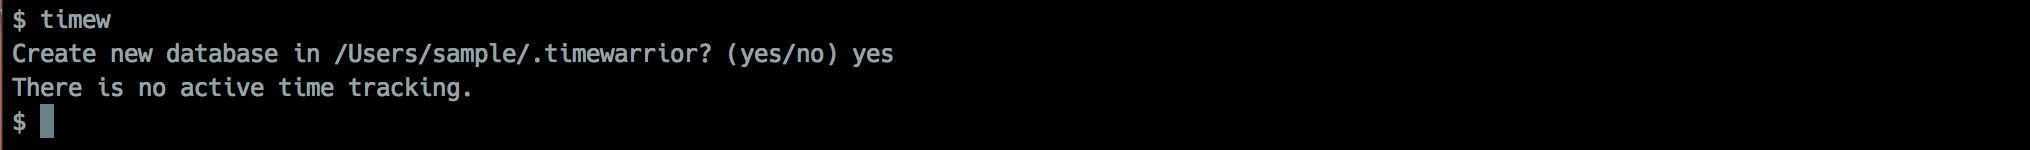
\includegraphics[width=12cm]{images/tutorial1.png}

    You are told that there is no active time tracking, and that's right, because we've done nothing yet.
\end{frame}

\begin{frame}[fragile]\frametitle{Data directory}
    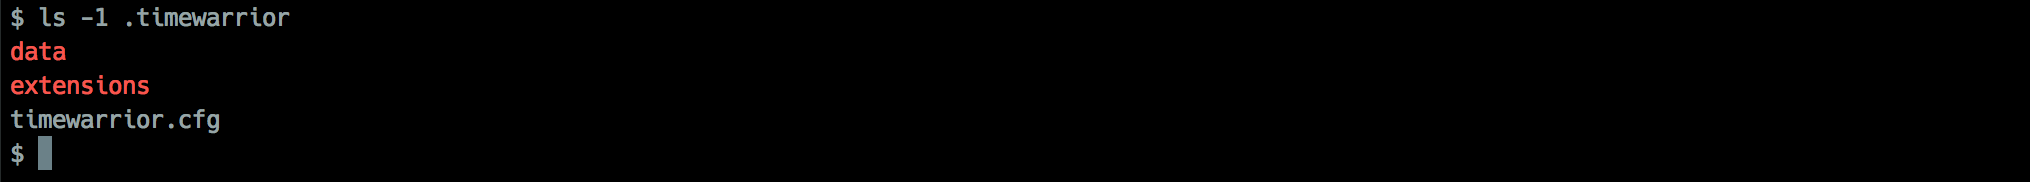
\includegraphics[width=12cm]{images/tutorial2.png}

    By default a \verb=.timewarrior= directory is created in your home directory, and contains a sub-directory for data, and another for extensions. There is also an empty configuration file created.

    Just like Taskwarrior, an empty configuration file means we are using all the default settings. If you want to use an alternate location, you can either symlink it to \verb=~/.timewarrior=, or use the \verb=TIMEWARRIORDB= environment variable to specify any location.
\end{frame}

\subsection{Stopwatch}

\begin{frame}[fragile]\frametitle{Stopwatch}
    The most basic tracking can be done by using the stopwatch features. Just like a stopwatch, you start and stop a clock, and you can see the elapsed time. Start the clock when you begin work work, and stop it when you are done. First let's see if the clock is running:

    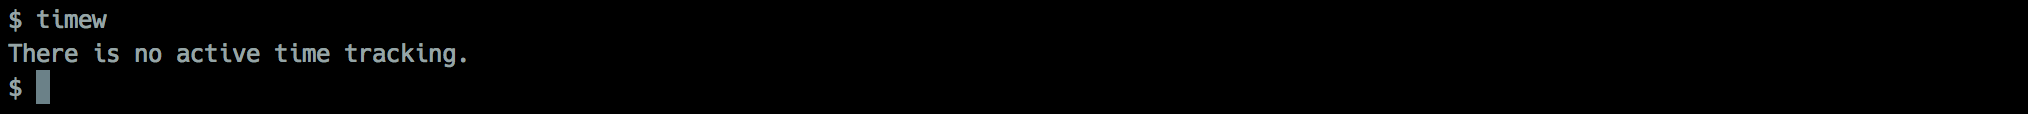
\includegraphics[width=12cm]{images/tutorial3.png}

    No it's not. You can always run timewarrior with no arguments to see if the clock is running, and no data is modified. Let's start the clock.

    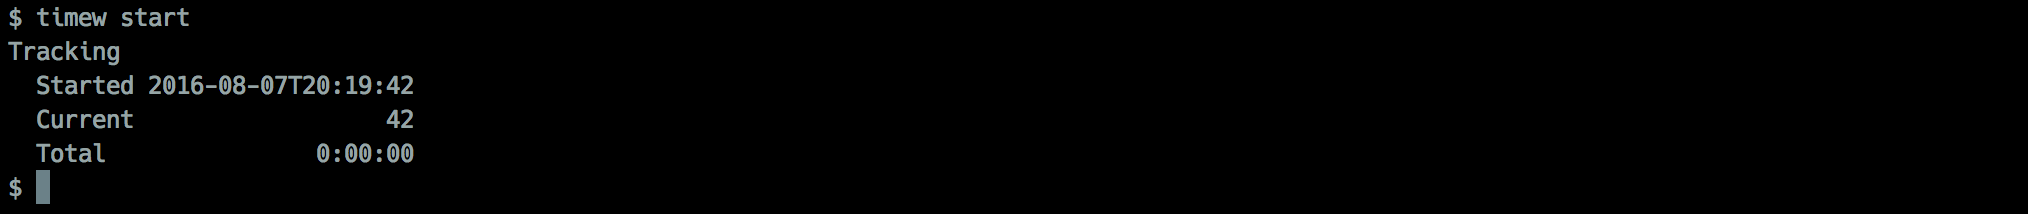
\includegraphics[width=12cm]{images/tutorial4.png}
\end{frame}

\begin{frame}[fragile]\frametitle{Stopwatch (2)}
    The clock is now running. In reality there is no clock and all that happened was that the start time was recorded, so don't be concerned about using system resources, as none are being used. Now when we check, we see a summary of the time recorded so far:

    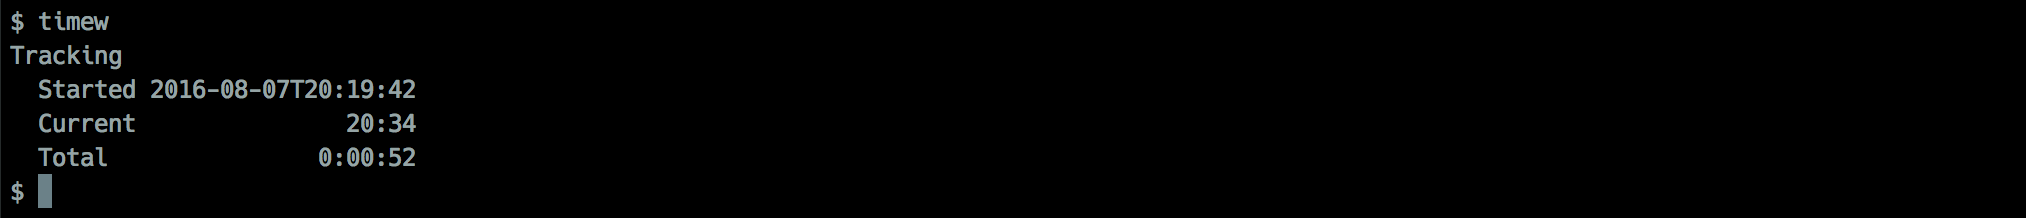
\includegraphics[width=12cm]{images/tutorial5.png}

    Once our work is complete, we stop the clock, and look at the summary.

    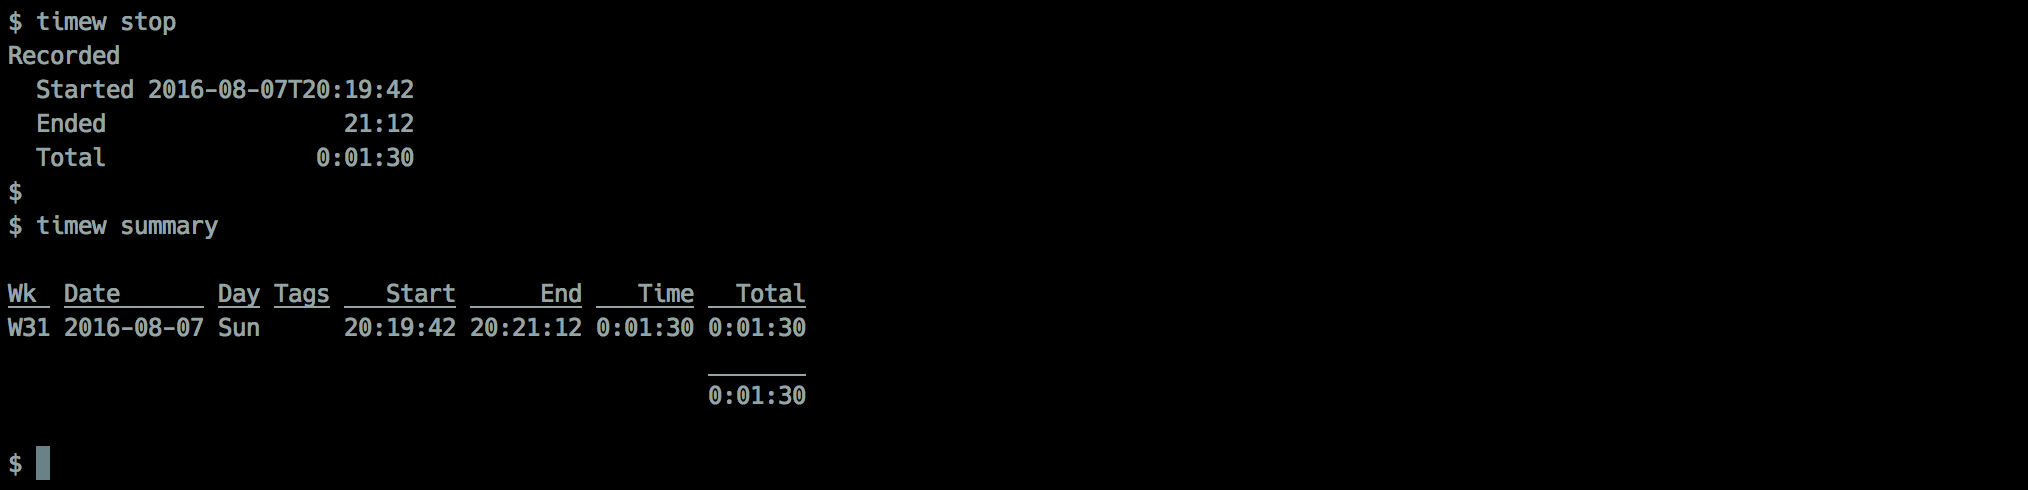
\includegraphics[width=12cm]{images/tutorial6.png}
\end{frame}

\begin{frame}[fragile]\frametitle{Stopwatch (3)}
    The summary report shows time that was tracked today by default.

    There is a \verb=continue= command that re-starts the previous tracking, and is useful if you stopped the clock during lunch, or overnight.

    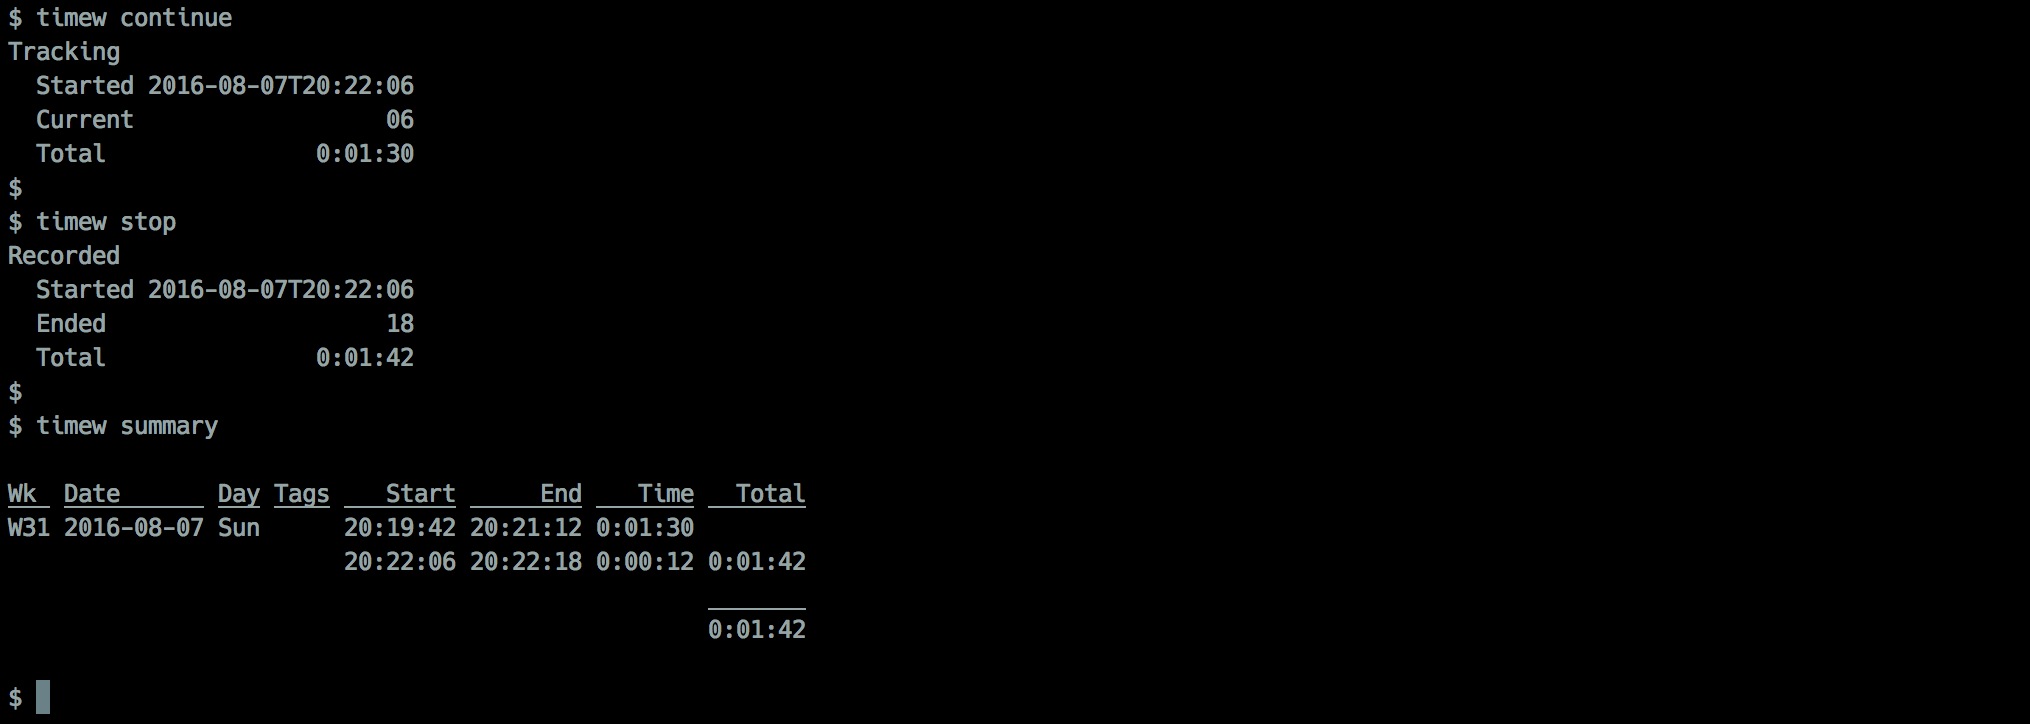
\includegraphics[width=12cm]{images/tutorial7.png}

    See how every time the clock is started, there is a new line in the \verb=summary= report?
\end{frame}

\begin{frame}[fragile]\frametitle{Stopwatch (4)}
    It is important to note that it is possible, and quite likely, that you will start the clock and leave it running by mistake. This is in fact one of the most annoying problems with any time tracking solution that relies on human interaction. While some tools will detect inactivity and stop the clock for you, Timewarrior does not. Instead it deals with this problem in two ways, first by making it easy to correct tracked time, and second by way of exclusions, which we will cover later.
\end{frame}

\subsection{Tags}

\begin{frame}[fragile]\frametitle{Tags}
    The examples so far did not use tags. Tags are optional, but when you do make use of tags, you start tracking time spent on \textit{different} activities.

    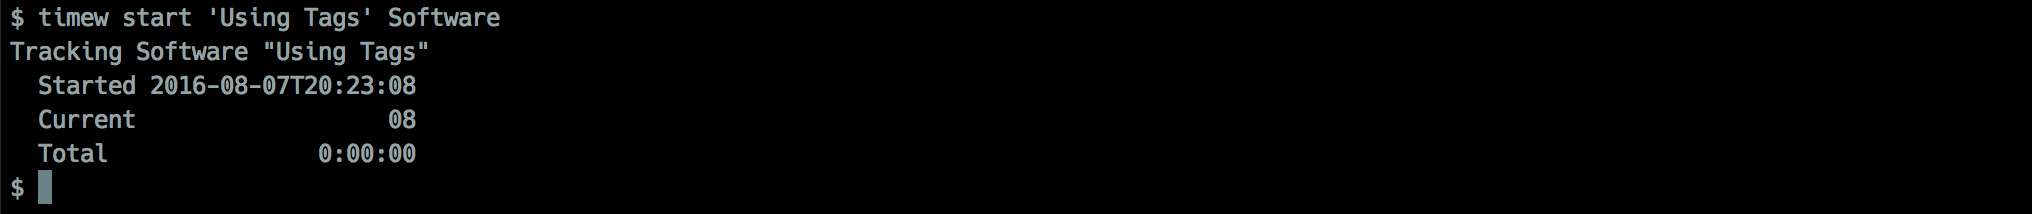
\includegraphics[width=12cm]{images/tutorial8.png}

    This example is tracking time using two different tags. The first is \textit{Using Tags}, the second is \textit{Software}. The first tag is two words, and because of the space between them, the quotes are needed to keep those two words together in one tag. The second tag is a single word and needs no quotes.
\end{frame}

\begin{frame}[fragile]\frametitle{Tags (2)}
    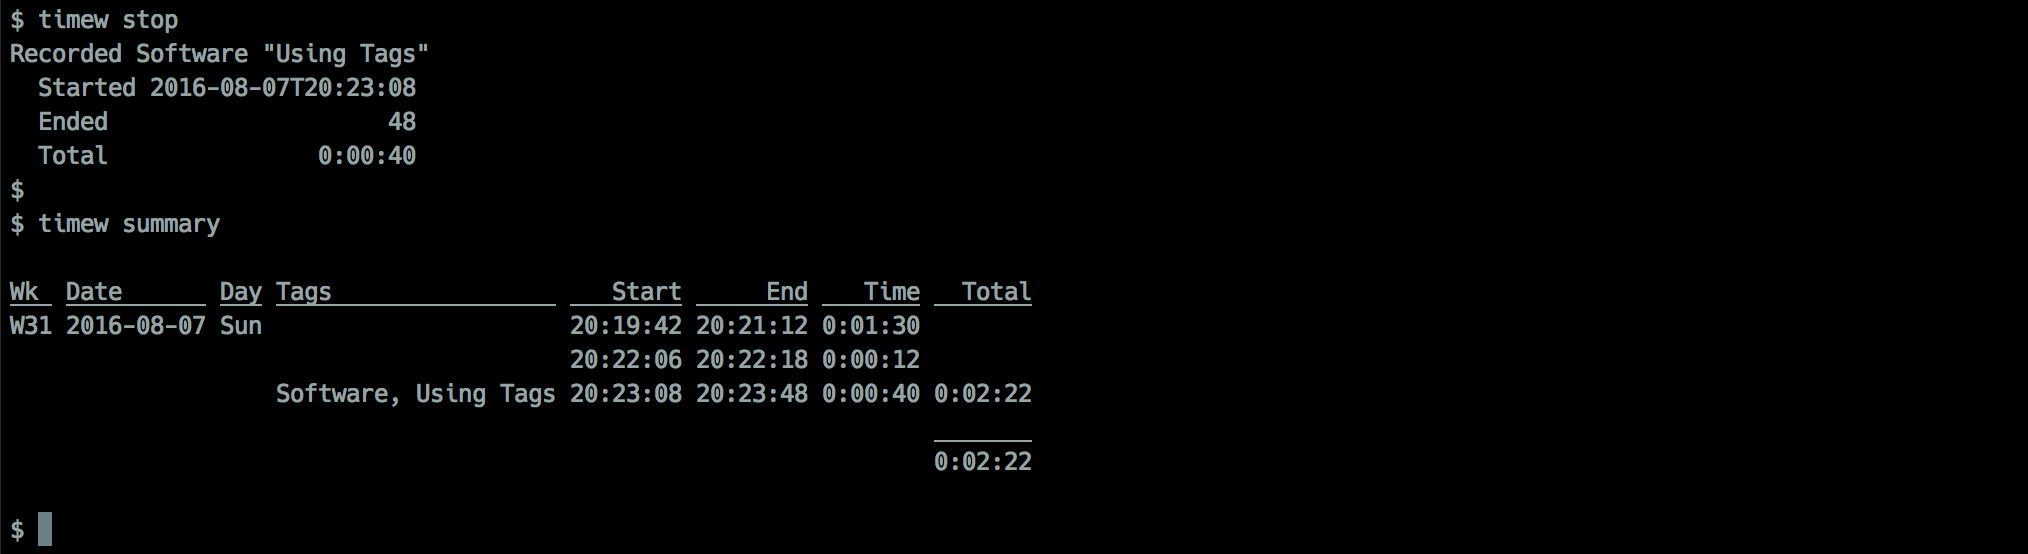
\includegraphics[width=12cm]{images/tutorial9.png}

    You can see that using tags is useful, but optional. Once you are using tags, you can use them to filter reports, such as the \verb=summary= report.

    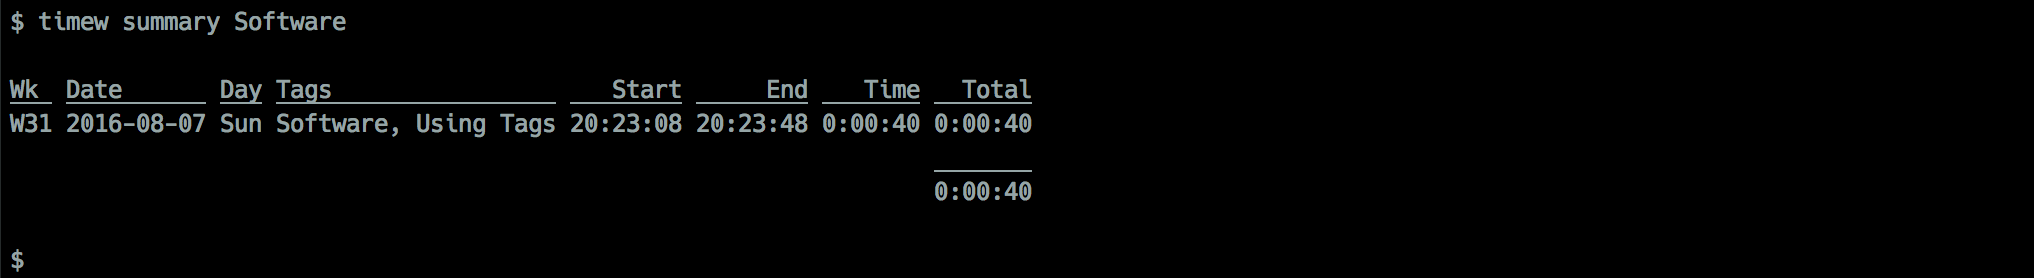
\includegraphics[width=12cm]{images/tutorial10.png}
\end{frame}

\begin{frame}[fragile]\frametitle{Tags (3)}
    There is a \verb=tags= command, which will show you all the tags you have used.

    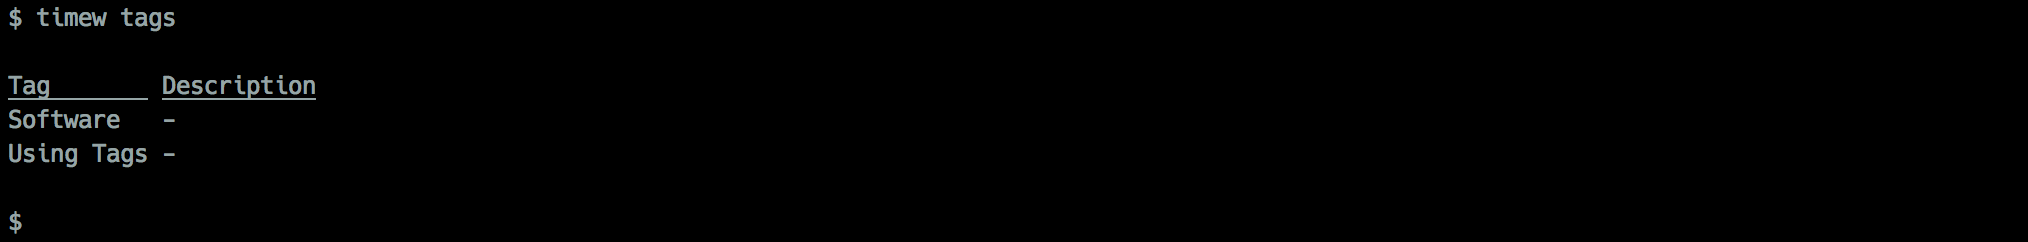
\includegraphics[width=12cm]{images/tutorial11.png}

    You may wonder how is that \textit{Description} column in the report used? It is the first example of tag metadata, which you can configure.

    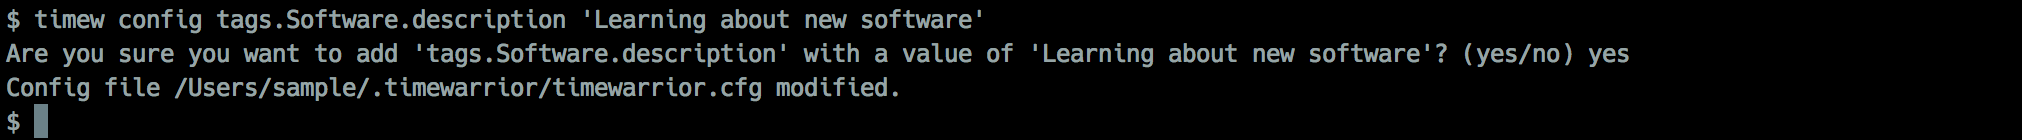
\includegraphics[width=12cm]{images/tutorial12.png}

    This is not currently used, but does represent how Timewarrior will be extended to include tag metadata in future releases.
\end{frame}

\subsection{Help}

\begin{frame}[fragile]\frametitle{Help command}
    Although we have just begun, it is important to mention the built-in help system. Let's look at the help for the \verb=continue= command.

    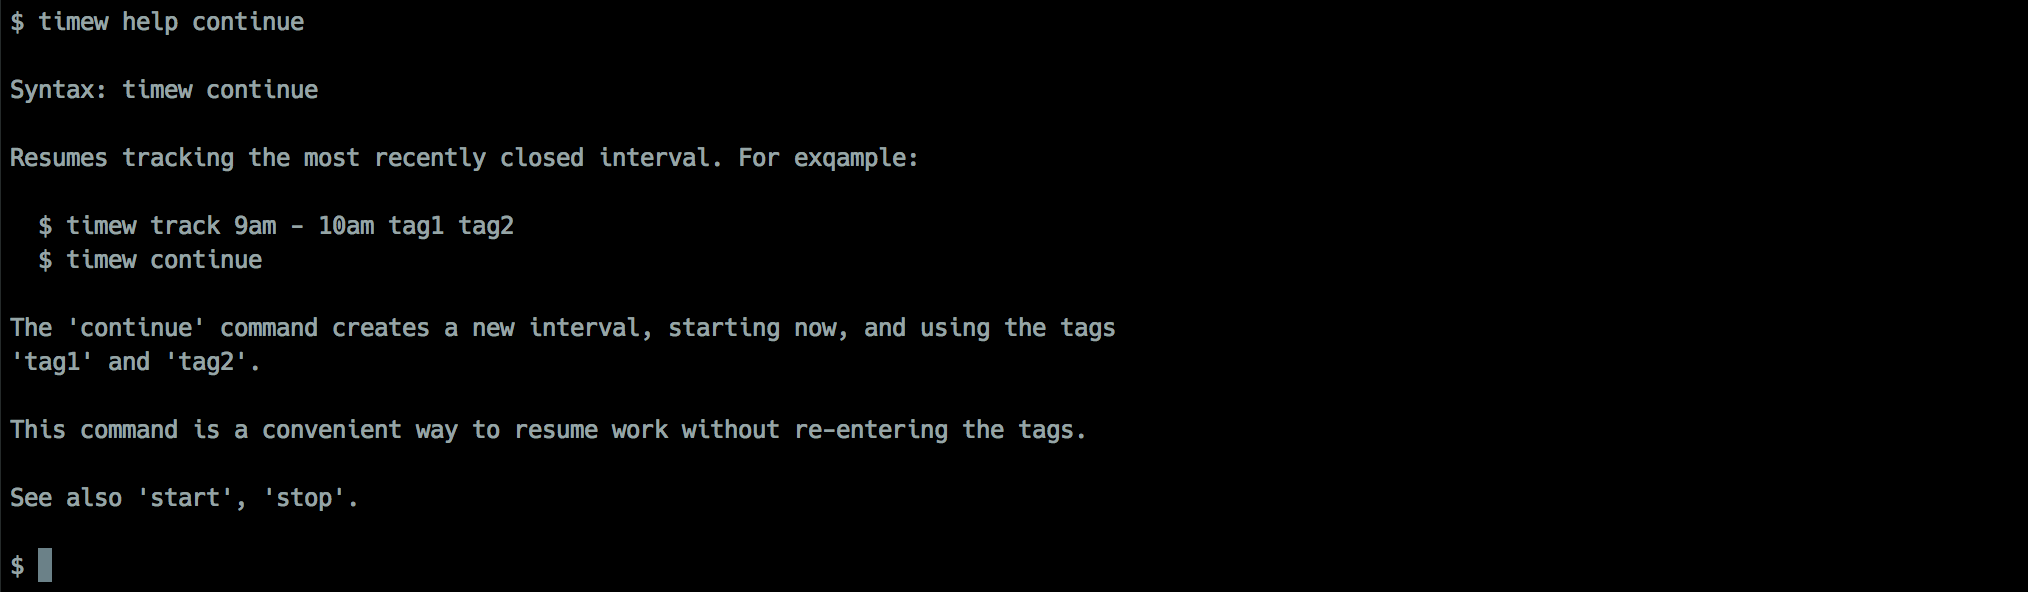
\includegraphics[width=12cm]{images/tutorial13.png}

    You can see that the help system contains examples, and introduces new commands and other help topics. From the help text, we learn that the \verb=continue= command will not only resume tracking but use the same set of tags.
\end{frame}

\begin{frame}[fragile]\frametitle{Man page}
    In addition to the built-in help, there is a man page which contains the same information plus a lot more.

    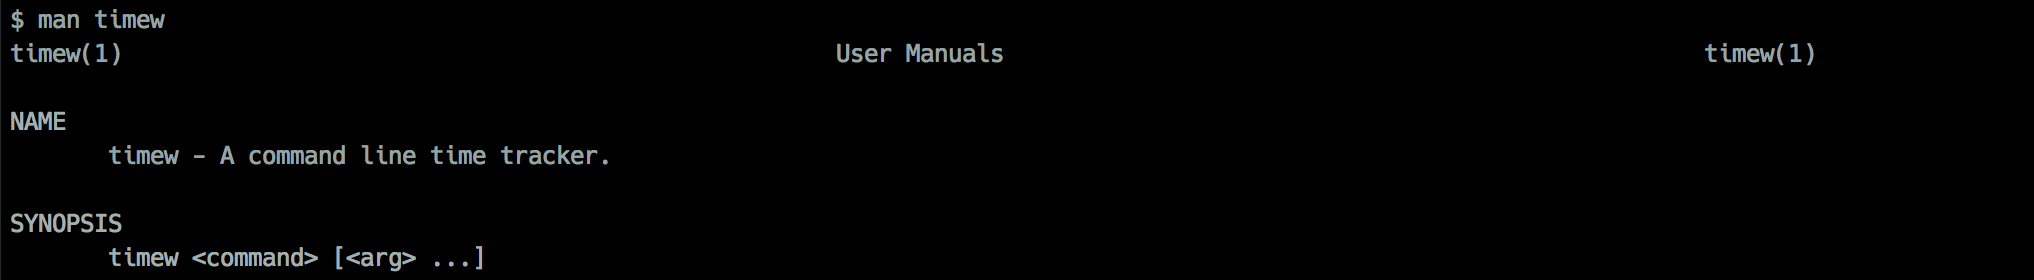
\includegraphics[width=12cm]{images/tutorial14.png}
\end{frame}

\subsection{Historical}

\begin{frame}[fragile]\frametitle{Historical}
    We have seen how to use the stopwatch feature, and combine it with tags. Additionally we can record time \textit{ex post facto}. So to track time I spent earlier in the day (but forgot to record), I use the \verb=track= command.

    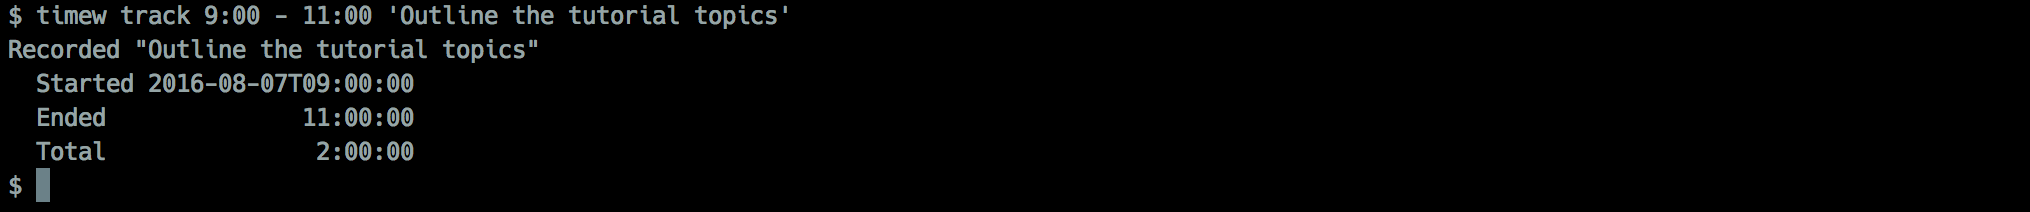
\includegraphics[width=12cm]{images/tutorial15.png}

    When Timewarrior sees a time like \verb=9:00= it always assumes it is in the past, because Timewarrior is a tool for recording what you have done or are doing, and is not a forward-looking planning tool.

    This is the opposite of Taskwarrior, which always looks forward, because tasks are generally going to be completed in the future.
\end{frame}

\begin{frame}[fragile]\frametitle{Historical(2)}
    There are other ways to specify time in the past, for example:

    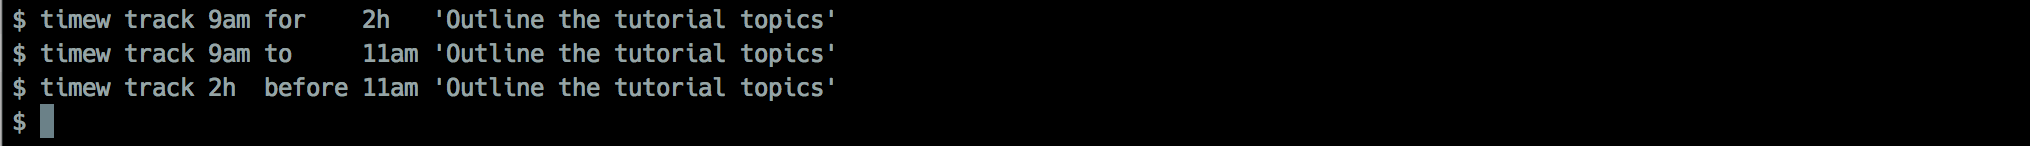
\includegraphics[width=12cm]{images/tutorial16.png}
\end{frame}

\begin{frame}[fragile]\frametitle{Historical(3)}
    And there are many more, which can be seen in the help system.

    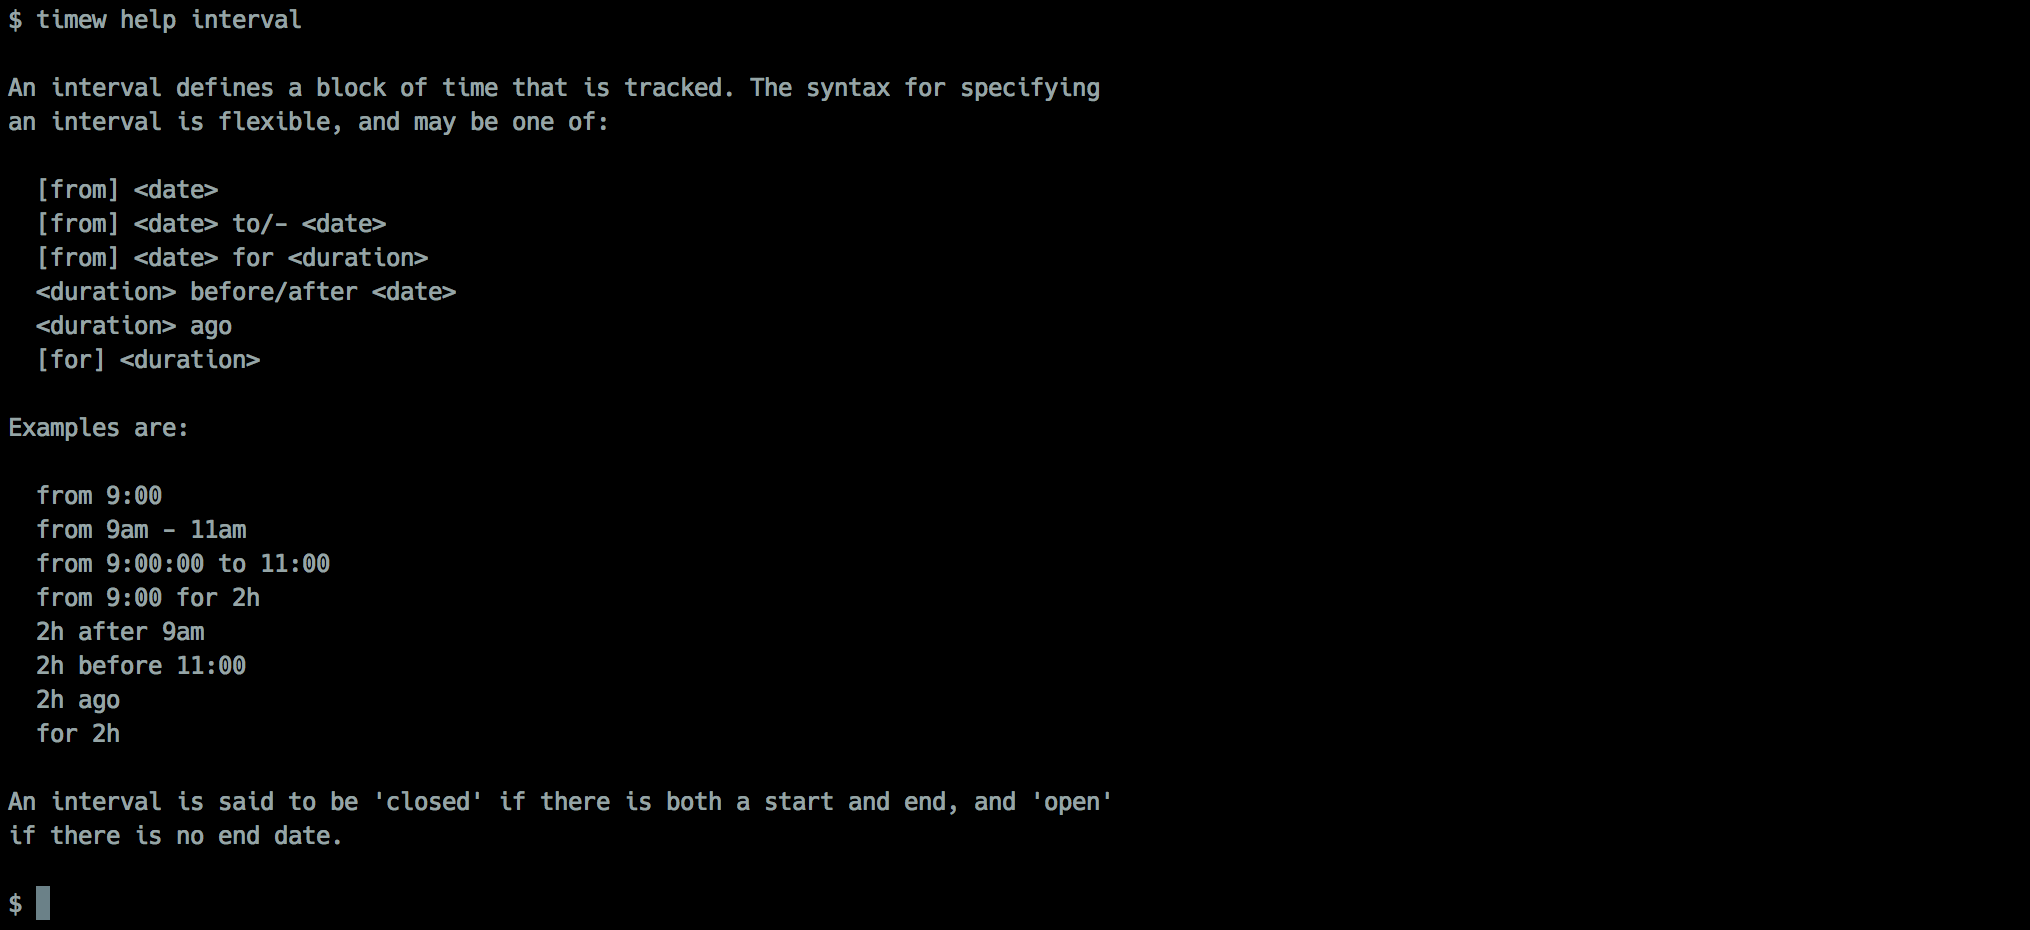
\includegraphics[width=12cm]{images/tutorial17.png}
\end{frame}

\begin{frame}[fragile]\frametitle{Historical(4)}
    In addition to time, you can specify date and time, so one equivalent command would use an ISO datetime.

    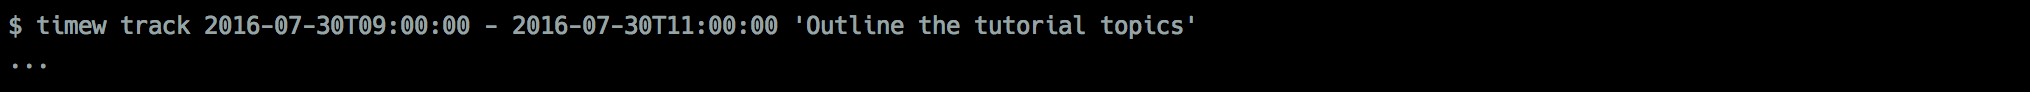
\includegraphics[width=12cm]{images/tutorial18.png}

    Again, you can see all the date formats listed using the help system.

    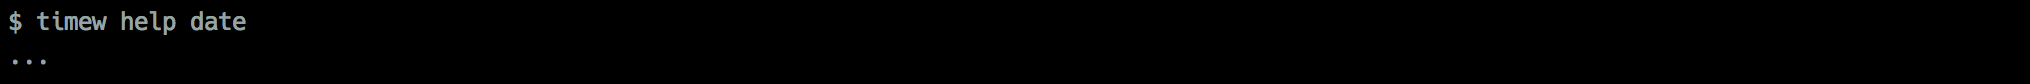
\includegraphics[width=12cm]{images/tutorial19.png}

    Using date synonyms you can track time for a whole month.

    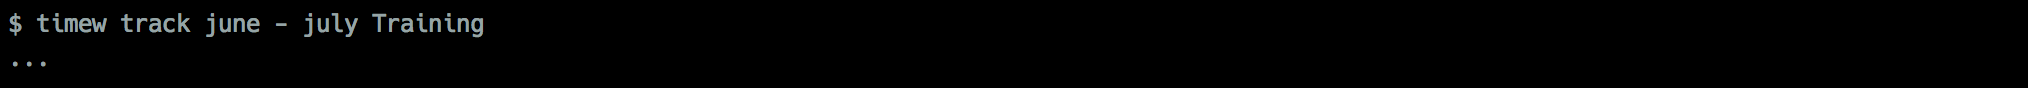
\includegraphics[width=12cm]{images/tutorial20.png}

    But that command will track all 30 days, all 24 hours each in June, including weekends, holidays and lunch breaks. Or does it? This is discussed later.
\end{frame}

\subsection{Hints}

\begin{frame}[fragile]\frametitle{Hints}
    Many commands support hints, which are words that start with a \verb=:= and are convenient representations to save time. Here is the \verb=:quiet= hint, being used to suppress all feedback:

    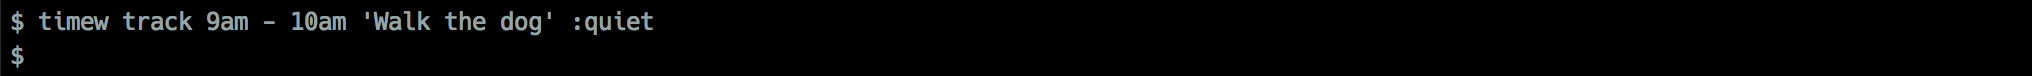
\includegraphics[width=12cm]{images/tutorial21.png}

    The \verb=:quiet= hint is the same as disabling verbosity, but is easier to specify, and temporary. Another hint is \verb=:yes=, which is used to override confirmation, by automatically answering \textit{yes} to the question.

    Some hints are shortcuts specifiers for date ranges. For example, the \verb=:yesterday= hint is a date range representing all day yesterday. Similarly, \verb=:lastweek= is also a date range. That makes the following two commands identical (assuming that today is the 6th):

    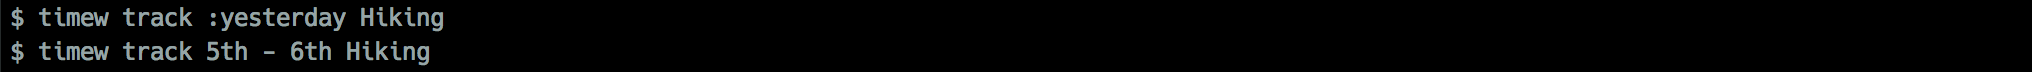
\includegraphics[width=12cm]{images/tutorial22.png}
\end{frame}

\begin{frame}[fragile]\frametitle{Hints (2)}
    The help system lists all the supported hints.

    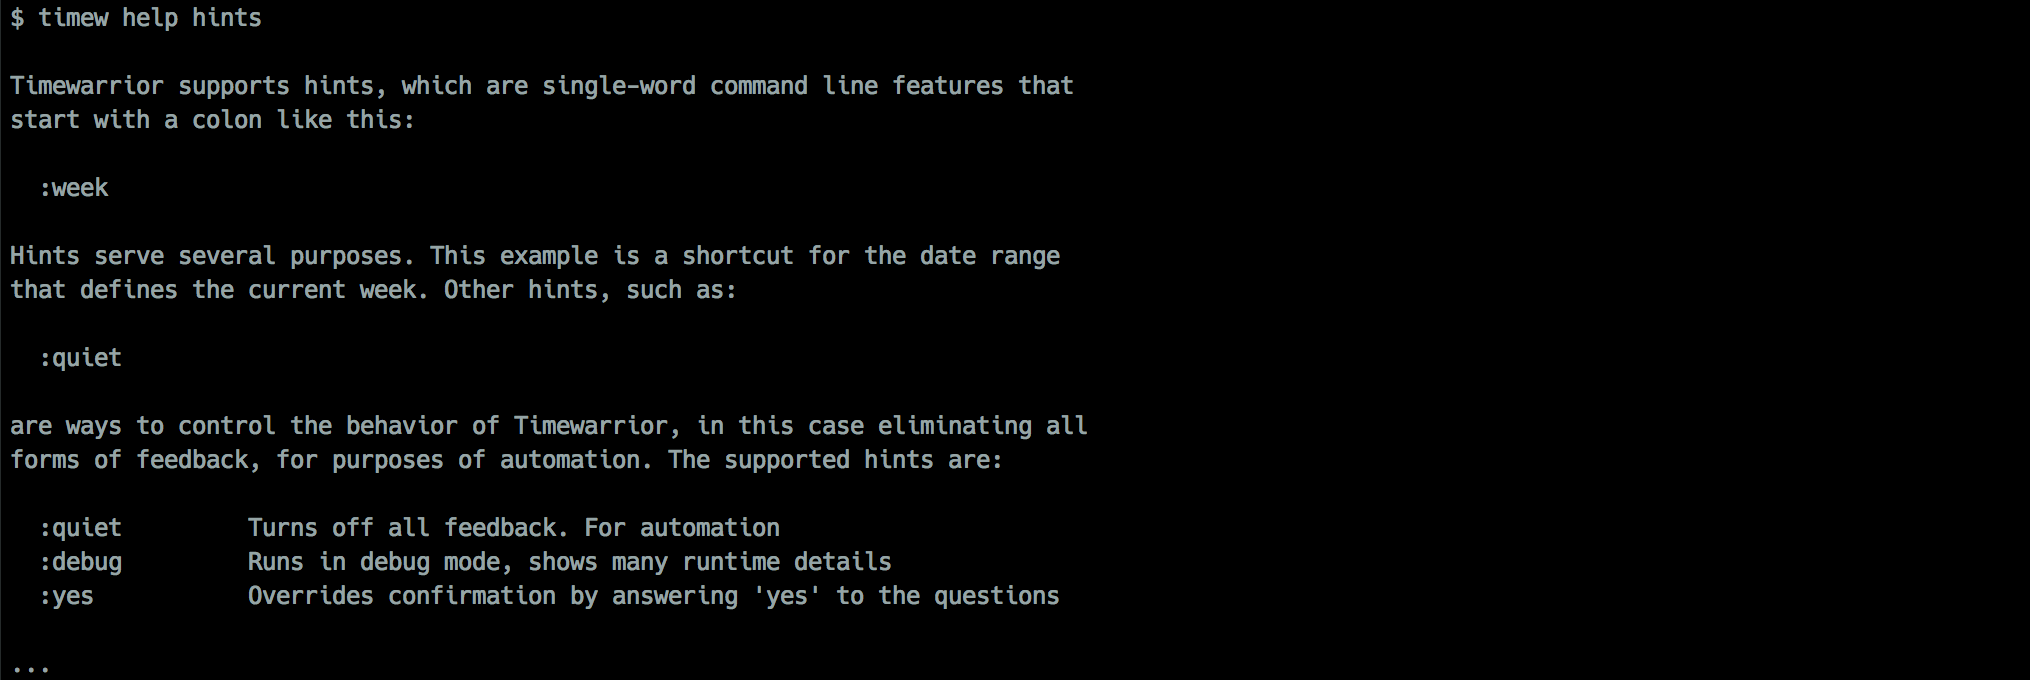
\includegraphics[width=12cm]{images/tutorial23.png}
\end{frame}

\subsection{Charts and Reports}

\begin{frame}[fragile]\frametitle{Charts}
    Timewarrior has a built-in chart that can show blocks of time by day. This is a text-based chart so it is not high resolution and has no drill-down capabilities. (Incidentally such a chart would be possible using the extension API, but by default, Timewarrior just has simple charting).

    There are three charts, which are really just three variations of the same chart, all controlled by configuration. We'll take a look at these charts, but first we need some sample data to look at.  Let us first track a couple of days of data, to illustrate how the charts work.

    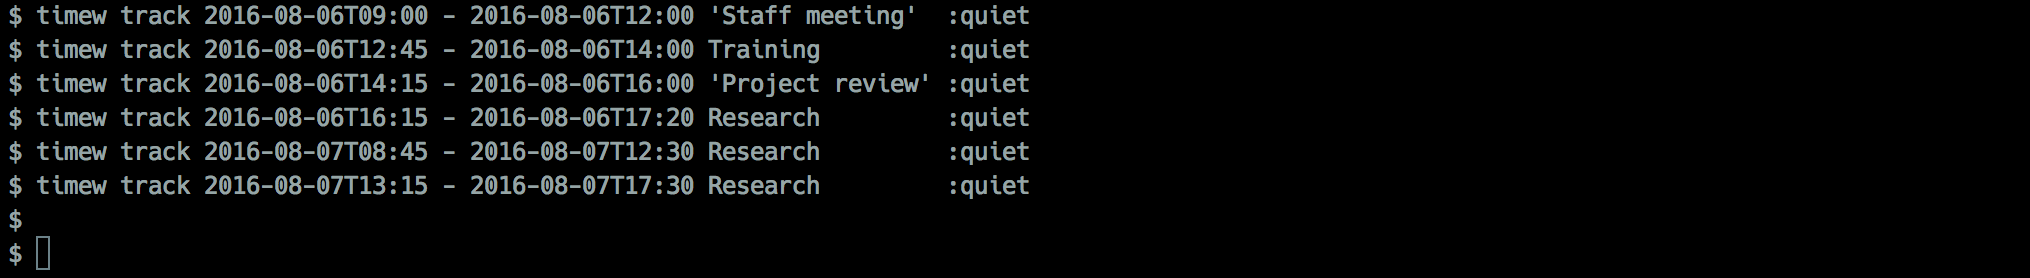
\includegraphics[width=12cm]{images/tutorial24.png}
\end{frame}

\begin{frame}[fragile]\frametitle{Charts (2)}
    We have tracked six separate intervals, and the summary report shows just that.

    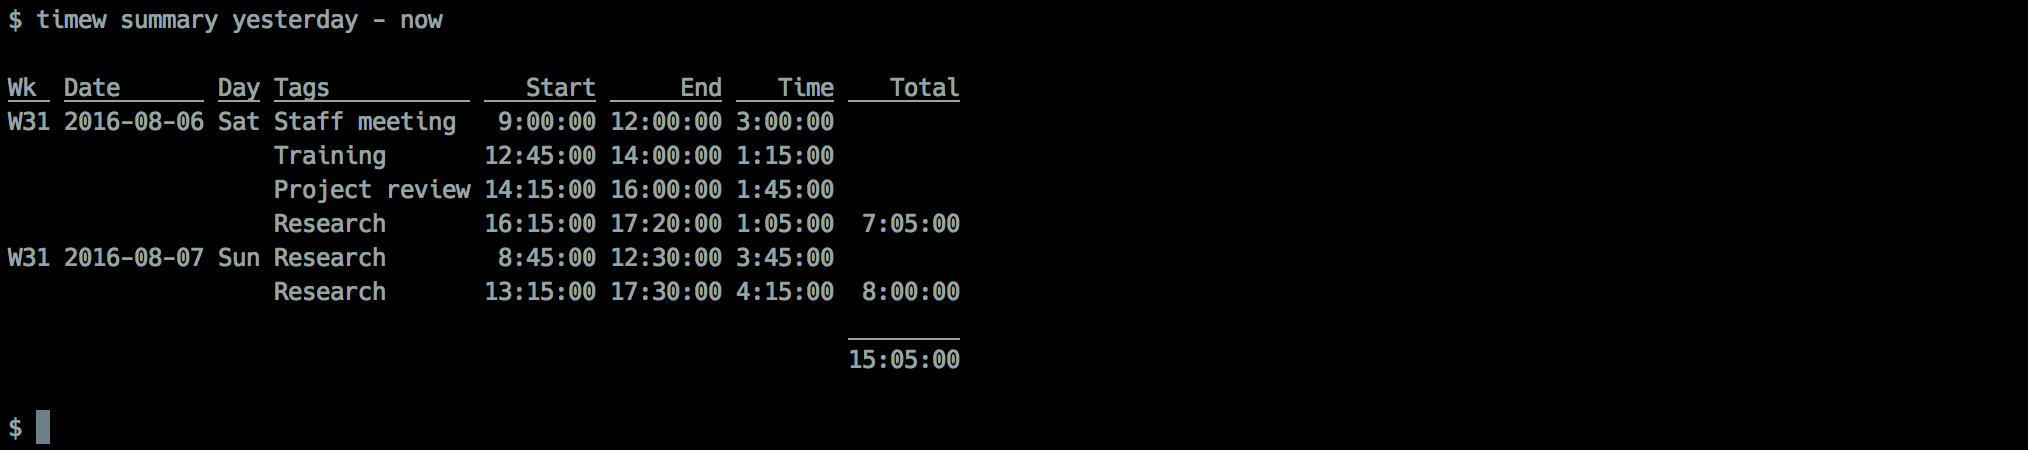
\includegraphics[width=12cm]{images/tutorial25.png}

    The summary report gives accurate time values, so this should be the preferred report for this reason. Let's look at the first chart, the \verb=day= report.

    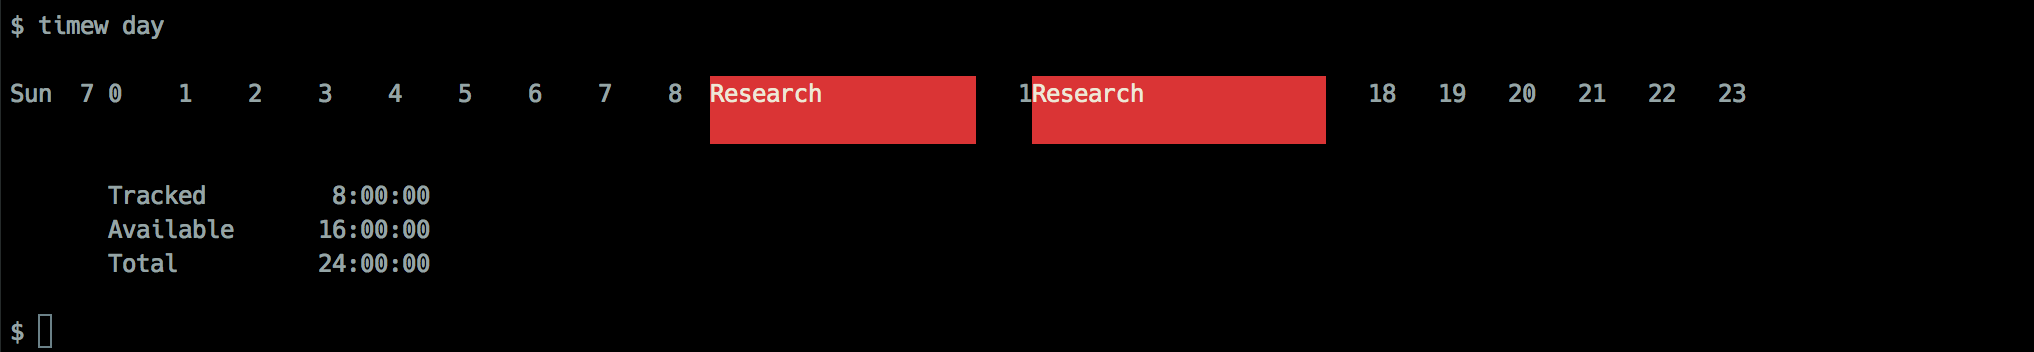
\includegraphics[width=12cm]{images/tutorial26.png}
\end{frame}

\begin{frame}[fragile]\frametitle{Charts (3)}
    Like the \verb=summary= report, the \verb=day= report shows data for today by default. You can make it show multiple days like this:

    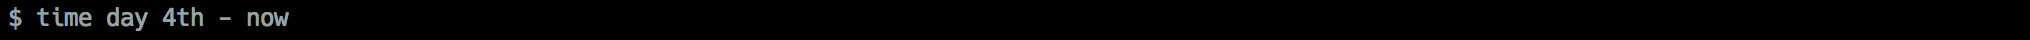
\includegraphics[width=12cm]{images/tutorial27.png}

    A better option is to use the \verb=week= report.

    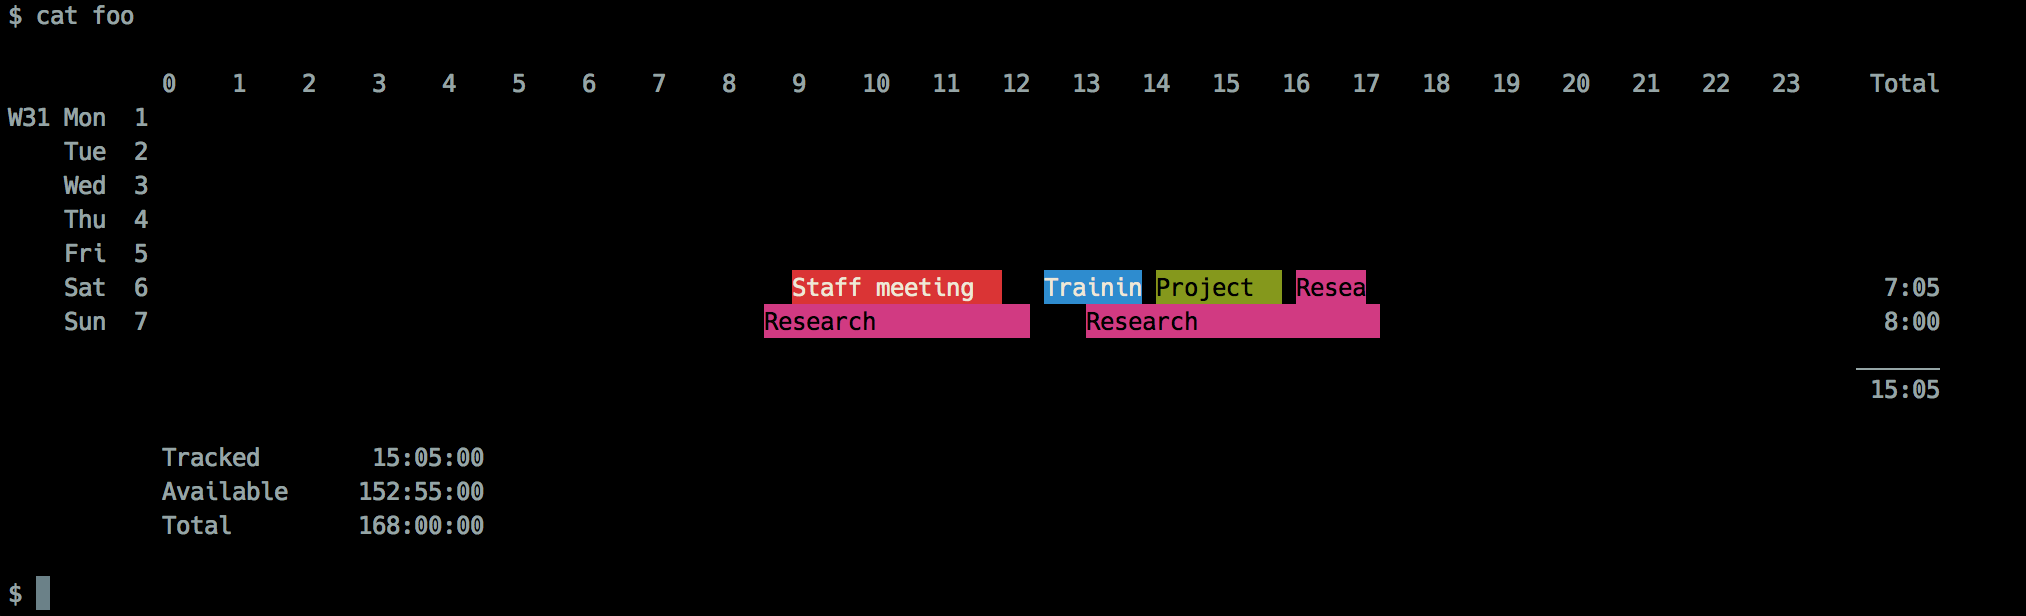
\includegraphics[width=12cm]{images/tutorial28.png}
\end{frame}

\begin{frame}[fragile]\frametitle{Charts (4)}
    There is also a \verb=month= report that looks the same, but is longer.

    Again, the only difference between these reports is configuration, and you can override any of this to customize these charts. See \verb=man timew= for full configuration details.
\end{frame}

\begin{frame}[fragile]\frametitle{Reports}
    We have seen the \verb=summary= and \verb=tags= reports, but there is another useful report that shows the untracked time in the day.

    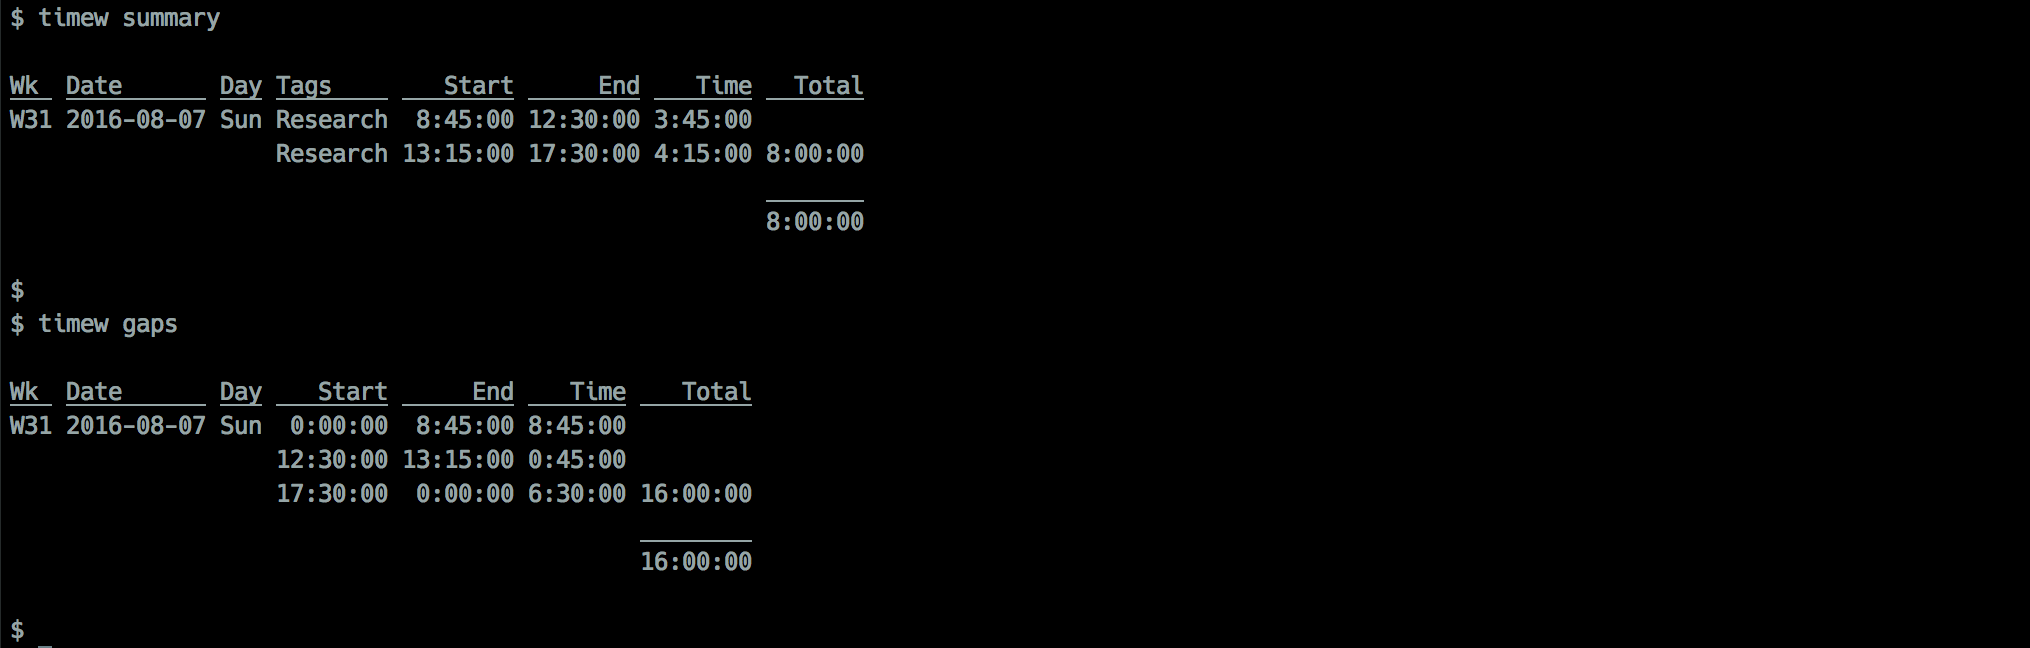
\includegraphics[width=12cm]{images/tutorial29.png}

    The \verb=gaps= report is useful for finding time in the day where you were not tracking time. In the example the gaps correspond well to time that was not spent working, so there is no need for adjustments.

    All reports in Timewarrior can be filtered by time interval and tags, but all have a default time interval.
\end{frame}

\subsection{Configuration}

\begin{frame}[fragile]\frametitle{Themes}
    Timewarrior has color themes that are mostly used by the charts to color the different parts of the display. To use a color theme, add this line to your \verb=~/.timewarrior/timewarrior.cfg= file with a text editor:

    \begin{lstlisting}
import /path/to/themes/dark_green.theme\end{lstlisting}

    Note that the path \verb=/path/to/themes= is a placeholder. Your installation will likely use a path more like this, but it should be noted that this path varies depending on platform and the wishes of the packager.

    \begin{lstlisting}
import /usr/local/share/doc/timew/doc/themes/dark_green.theme\end{lstlisting}

    There are a few simple themes available initially, but this collection will grow and improve. Timewarrior is also likely to make greater use of themes in future releases.
\end{frame}

\begin{frame}[fragile]\frametitle{Holidays}
    Timewarrior can also make use of Holiday files. In the same way that a color theme was imported into the configuration file, a holiday file can also be used:

    \begin{lstlisting}
import /usr/local/share/doc/timew/doc/holidays/holidays.en-US\end{lstlisting}

    Again, that path is platform-dependent, so use the appropriate path for your system.

    When a holiday file is used, Timewarrior knows that there are some days in the year that are not work days. While this changes nothing about your ability to track time, it does affect some automatic tracking features, which we will cover next.

    There is a \verb=README= document and a \verb=refresh= script provided with the holiday file, which explains how to update the holiday data, and how to obtain holiday files for other locales. Note that only the \verb=en-US= locale is included by default.
\end{frame}

\begin{frame}[fragile]\frametitle{Exclusions}
    Exclusions are a very powerful Timewarrior feature, and make automatic time tracking possible. An exclusion -- much like a holiday -- represents a block of time where you do not expect to work.

    The simplest exclusion is a day off work. Suppose you took a day off, on August 4th. You can define this day as an exclusion.

    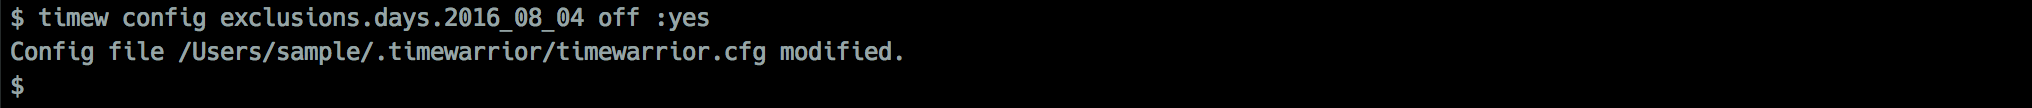
\includegraphics[width=12cm]{images/tutorial30.png}
\end{frame}

\begin{frame}[fragile]\frametitle{Exclusions (2)}
    The date must be formatted in this precise way. Note the use of the \verb=:yes= hint to override confirmation. Now we see on the \verb=week= report that the day is marked as non-working.

    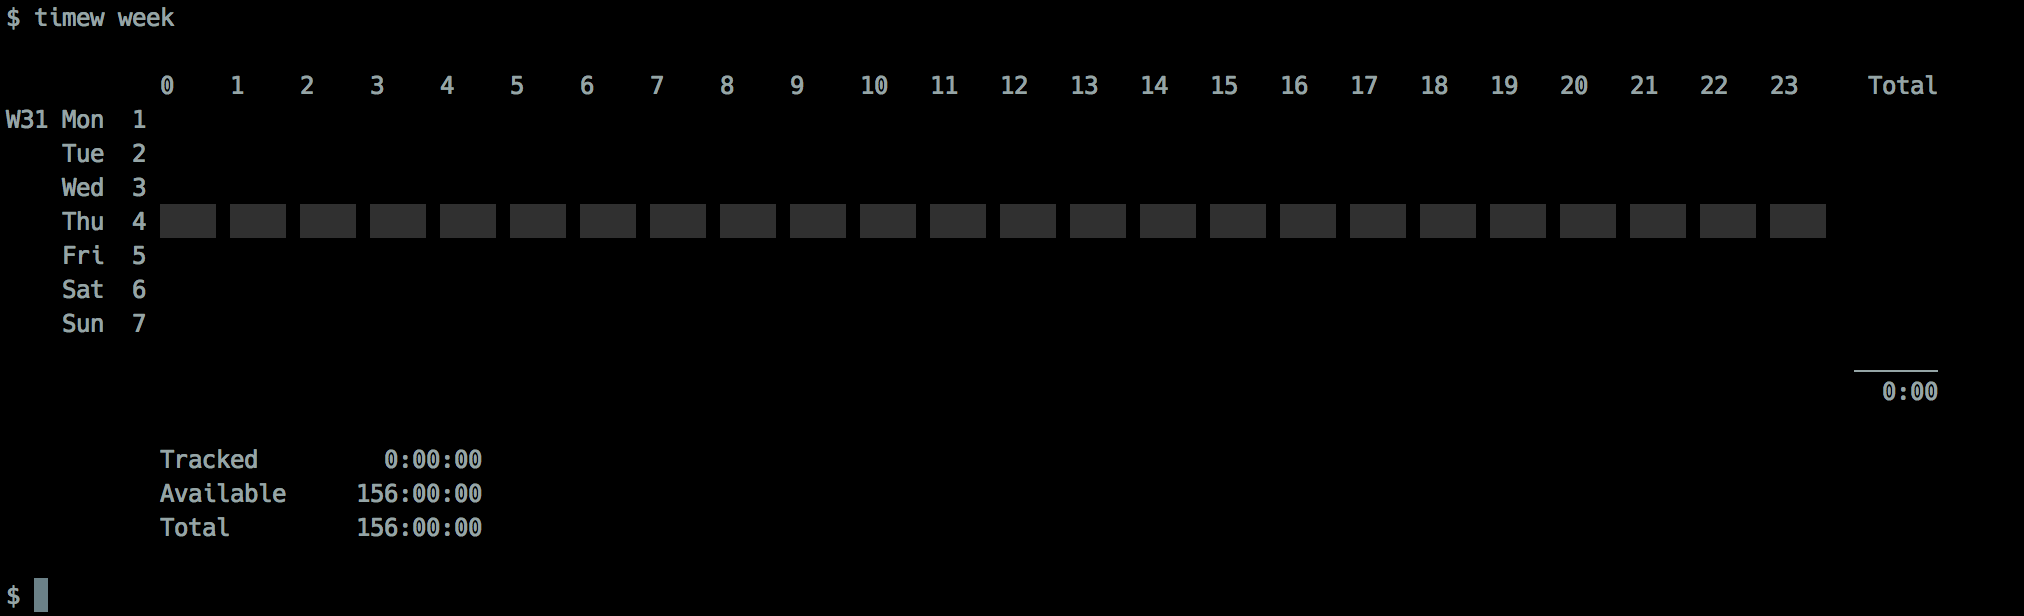
\includegraphics[width=12cm]{images/tutorial31.png}
\end{frame}

\begin{frame}[fragile]\frametitle{Exclusions (3)}
    Similarly, if you worked on a holiday, you can define that day as a work day, and therefore available for automatic tracking.

    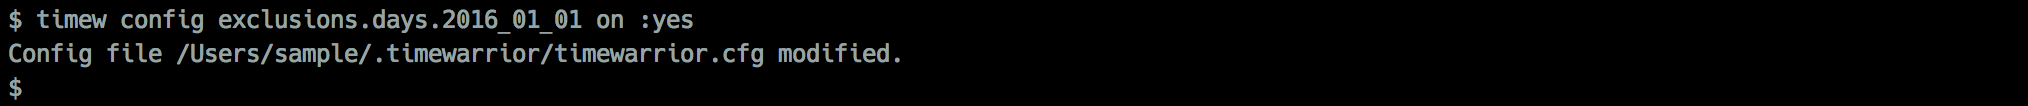
\includegraphics[width=12cm]{images/tutorial32.png}

    Here we have (re)defined January 1st as a working day, which was previously defined as a holiday in the \verb=en-US= locale.
\end{frame}

\begin{frame}[fragile]\frametitle{Exclusions (4)}
    In addition to whole days working or not working, you can define exclusions for each day of the week to represent your work schedule. Suppose you work a regular weekly schedule, that starts at 8:30am, Monday to Friday, with weekends off. You take a 45-minute lunch break each day, and leave work at 5:30pm. On Fridays you leave early.

    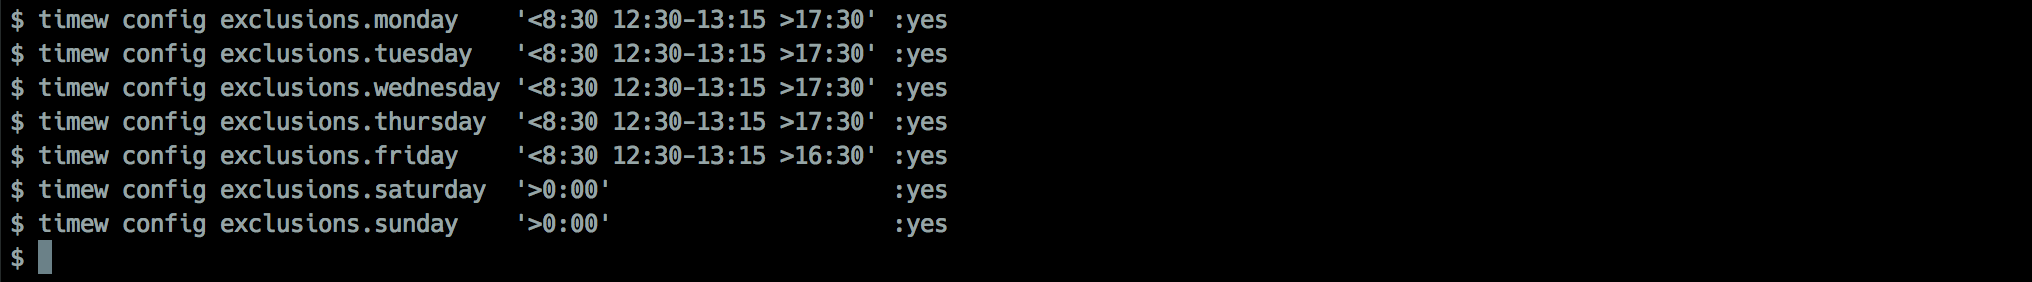
\includegraphics[width=12cm]{images/tutorial33.png}
\end{frame}

\begin{frame}[fragile]\frametitle{Exclusions (5)}
    You can view this in the \verb=week= report, and here we will use the \verb=:blank= hint to remove all the tracked data from the report, leaving only the exclusions.

    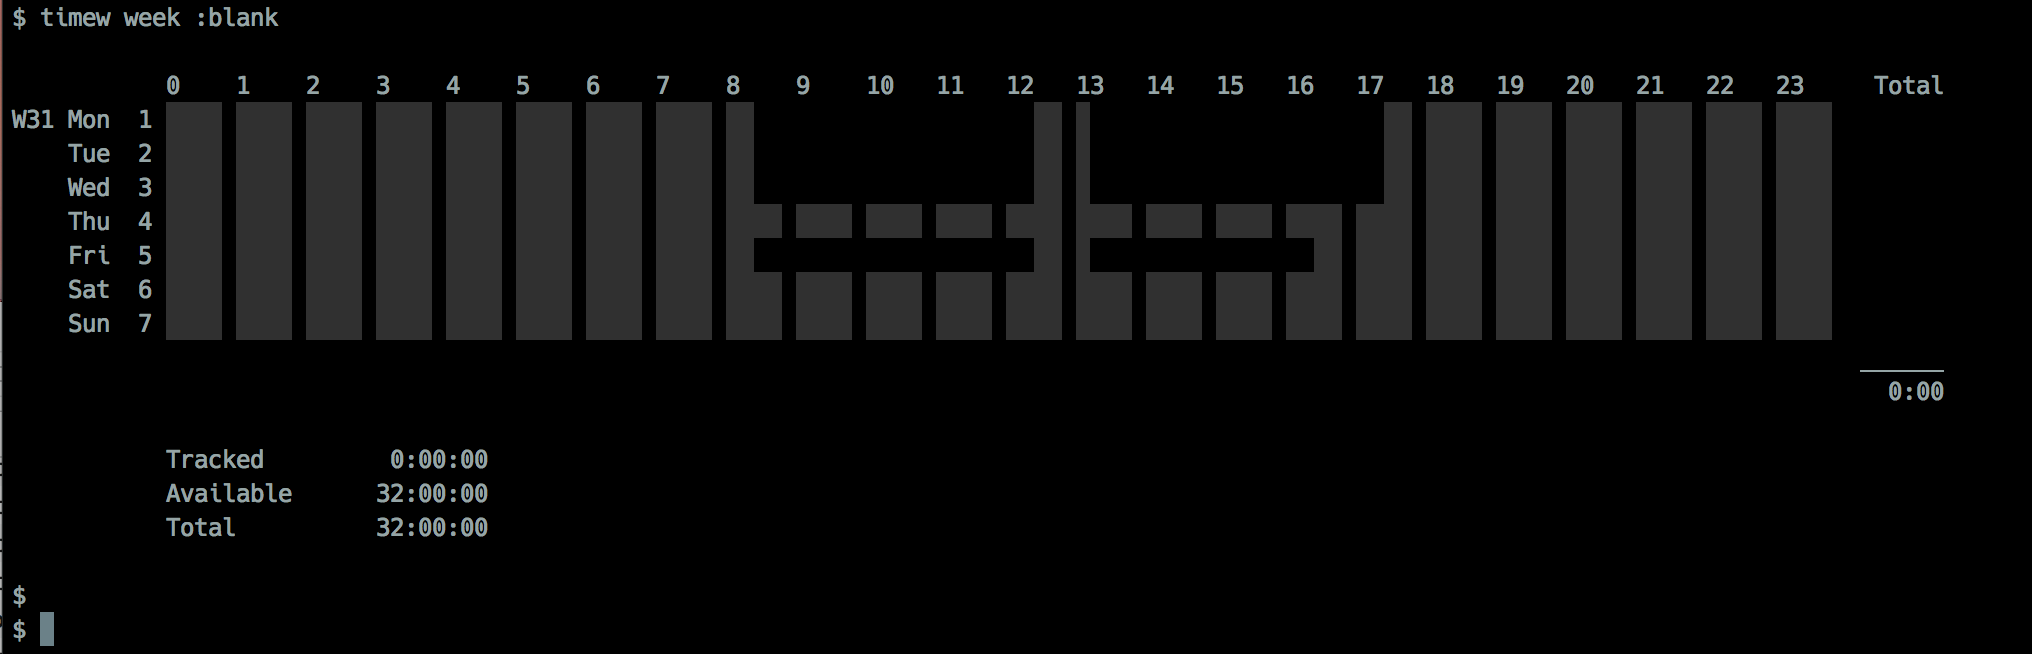
\includegraphics[width=12cm]{images/tutorial34.png}

    Your whole work week is defined. While you are not at all constrained by this defined schedule, it does control automatic time tracking.
\end{frame}

\begin{frame}[fragile]\frametitle{Automatic Tracking}
    Once you have defined exclusions for your workweek, the tracked time will conform to the set boundaries. Suppose this is our work week:

    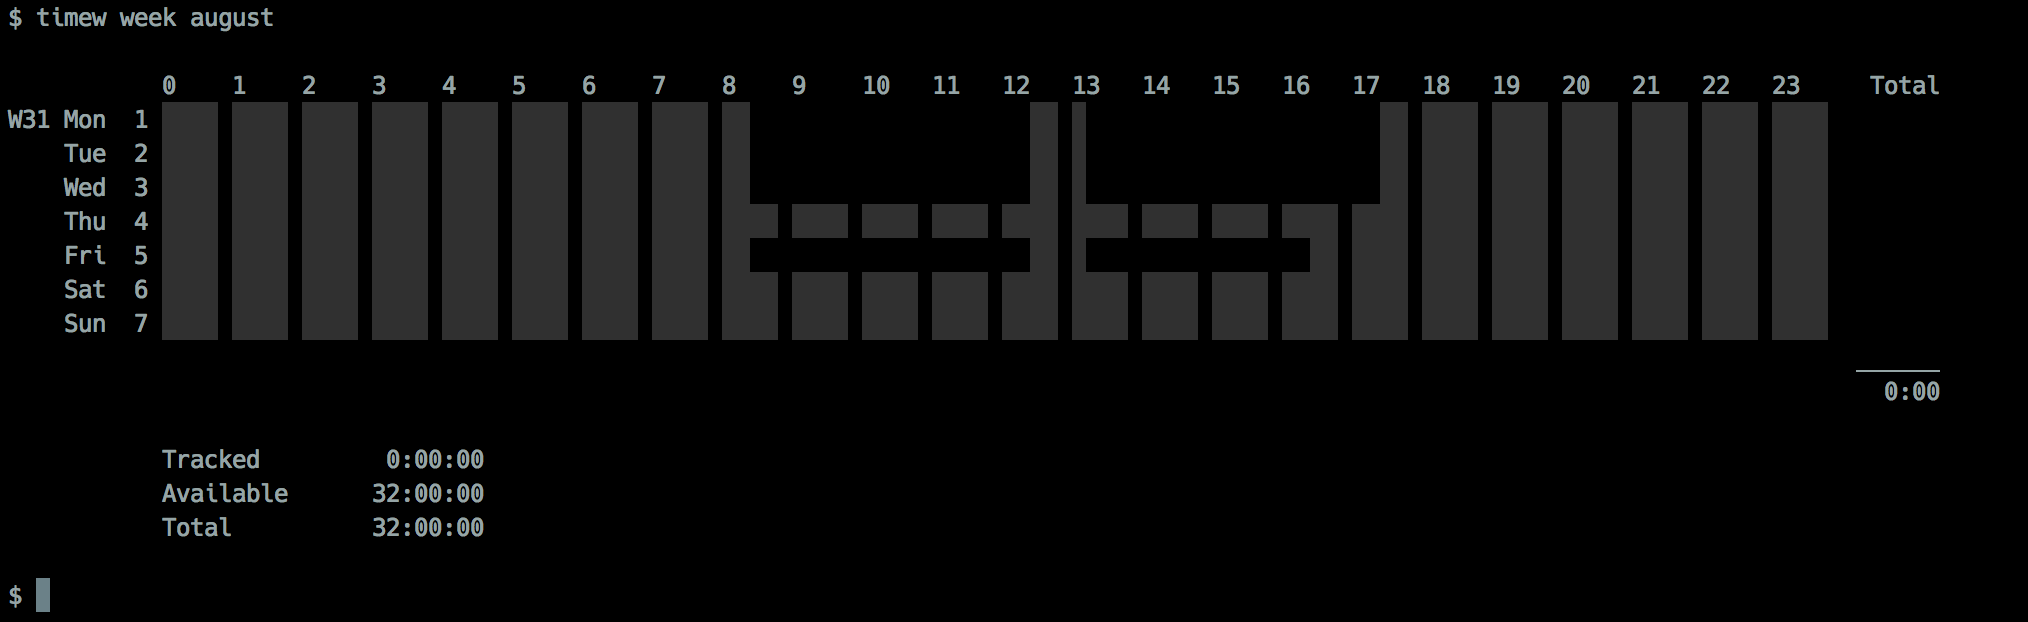
\includegraphics[width=12cm]{images/tutorial35.png}
\end{frame}

\begin{frame}[fragile]\frametitle{Automatic Tracking (2)}
    There is no tracked time, but there are 40:15:00 hours available to be tracked.  If we worked the whole week on our \textit{Research} project, we can track all that time with one command:

    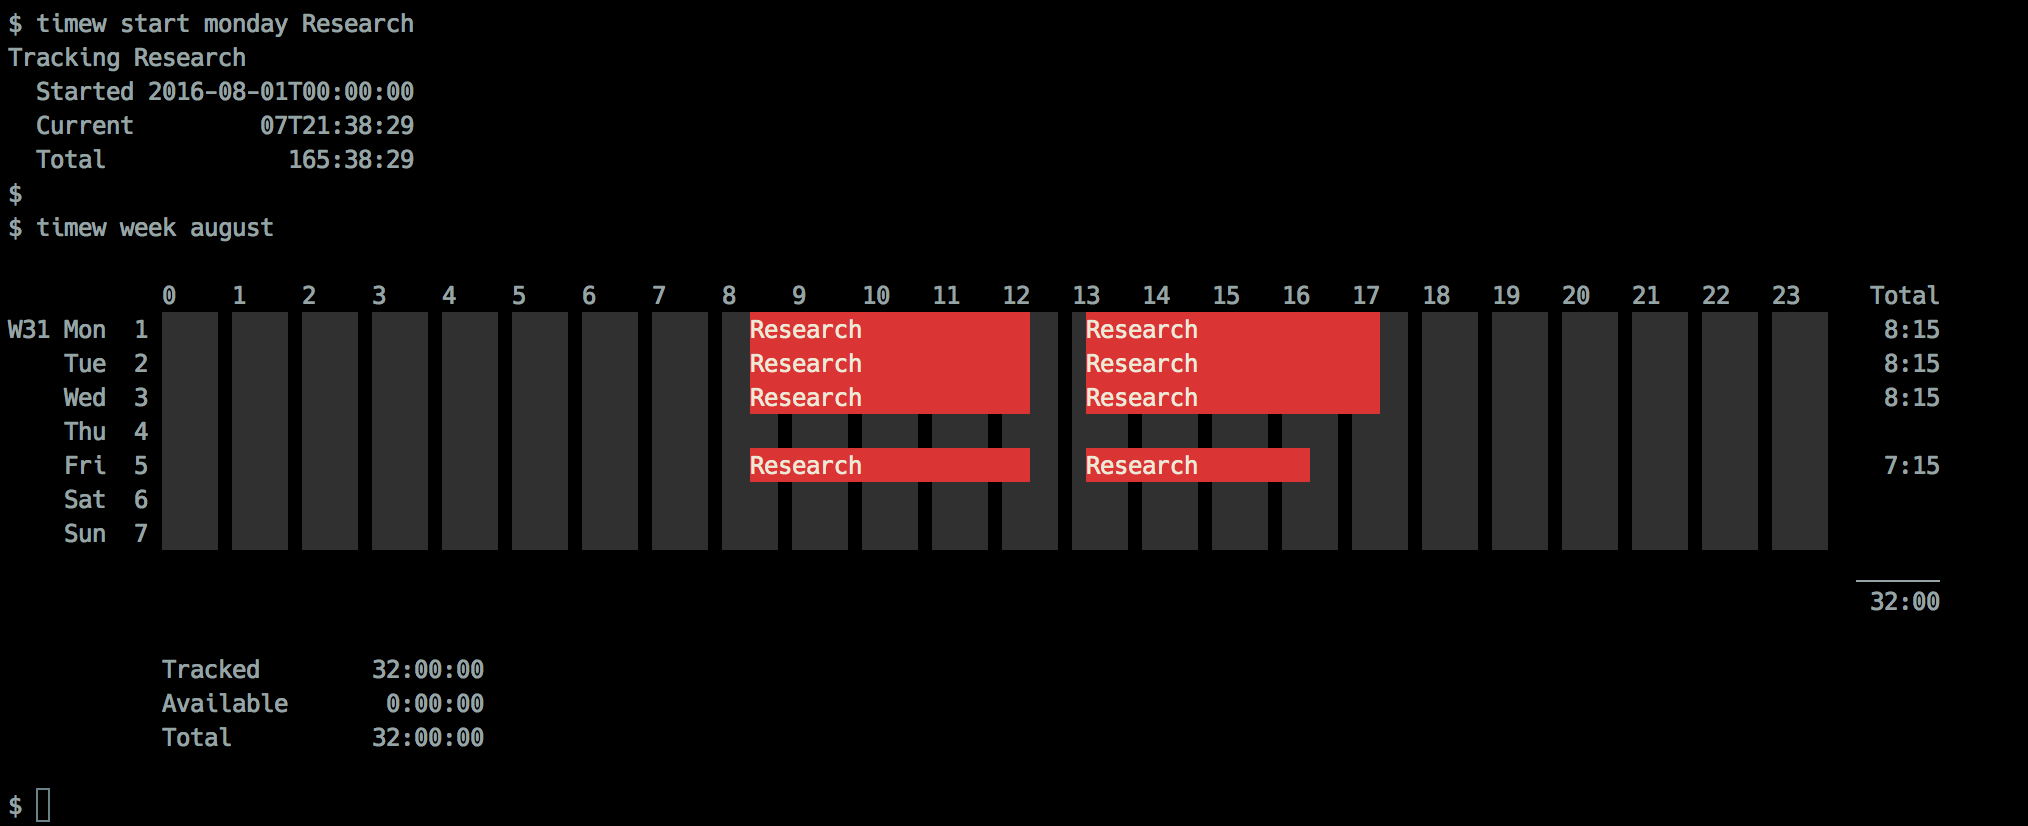
\includegraphics[width=12cm]{images/tutorial36.png}

    We see that the exclusions are automatically subtracted from the time, and fill the whole week, leaving no available time.

    Note that this example tracks up until \textit{now}, and as this tutorial is being written on a weekend, you can see that the tracking stops on Friday, and does not continue into the weekend.

    If this was being done on the Friday, at 16:23, then the \verb=week= report would stop precisely at 16:23, because it is an open interval.
\end{frame}

\section{Corrections}

\begin{frame}[fragile]\frametitle{Corrections}
    With or without the use of exclusions, there is always the need to make corrections to the tracked time. As mentioned earlier, it is quite likely that the clock would be left running by mistake, or that the tracking was started or stopped at the wrong time. We will create some incorrect time tracking, and then correct it.

    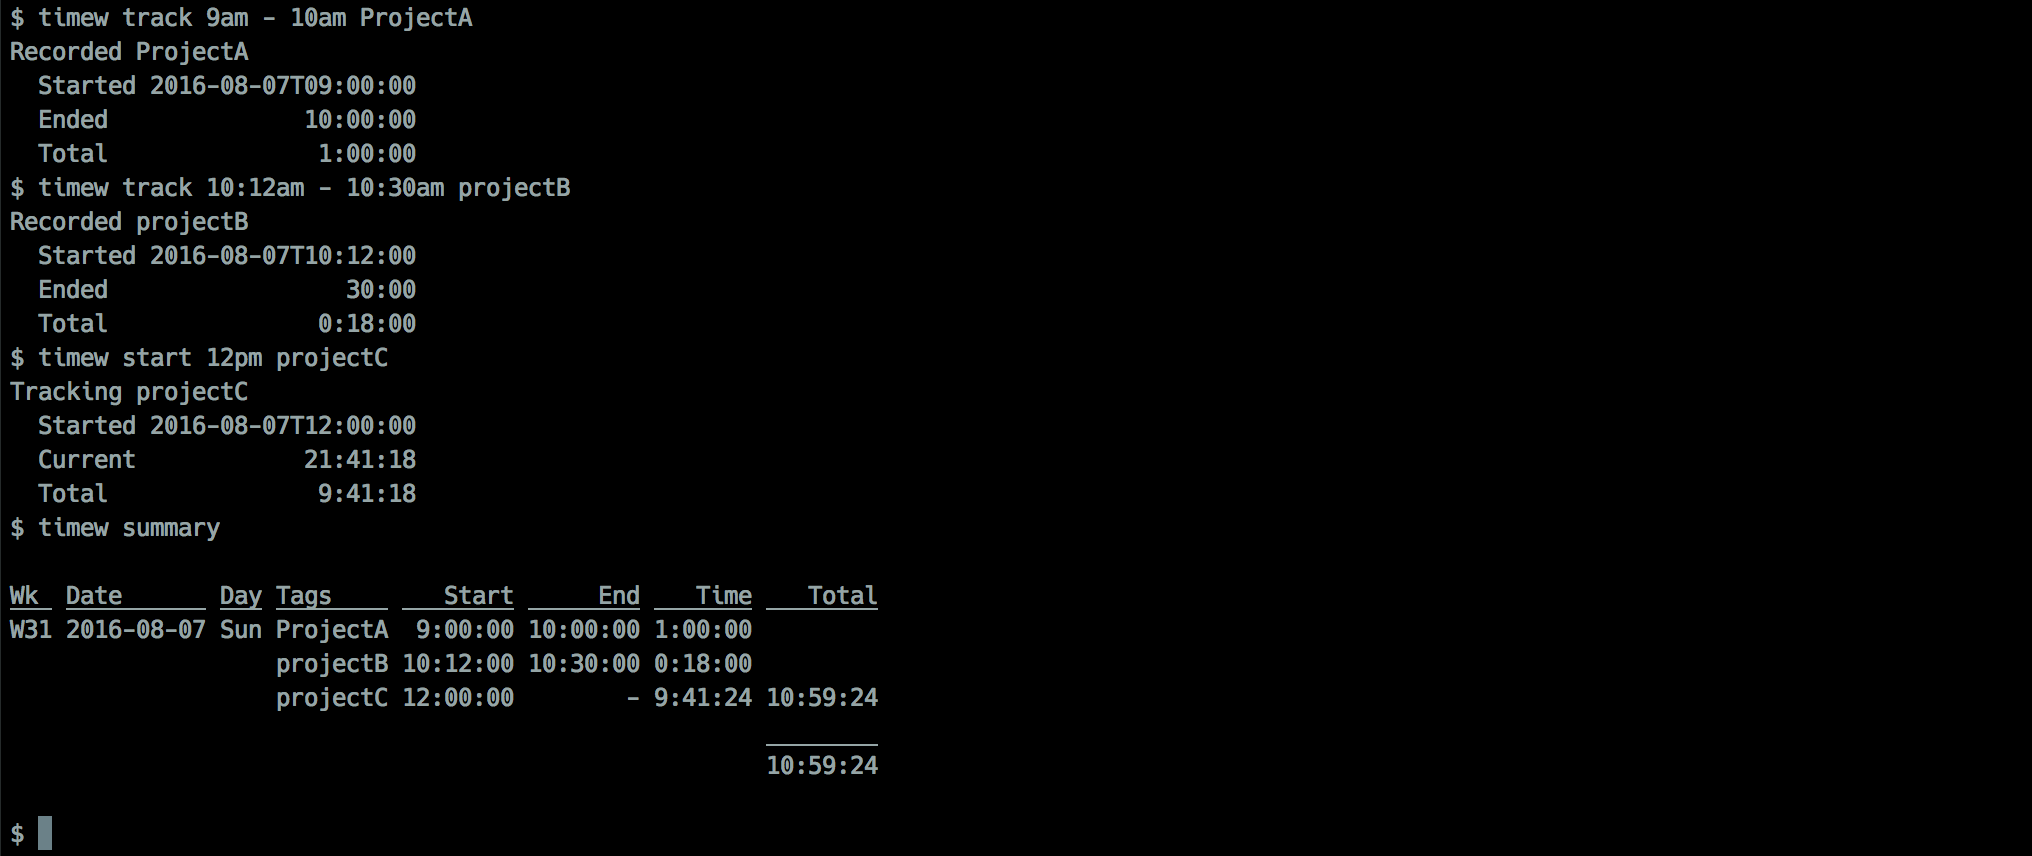
\includegraphics[width=12cm]{images/tutorial37.png}
\end{frame}

\begin{frame}[fragile]\frametitle{Corrections (2)}
    I actually started work at 8:30am, but forgot to start the clock at the beginning. I also did not take a break at 10am, I again forgot to start the clock. Then I was working on projectC since about 11am, but didn't record it properly.

    These are typical mistakes, and are easy to fix, as there are several commands for making adjustments like this.

    To make an adjustment to an interval, we need first to identify that interval. The \verb=summary=, \verb=day=, \verb=week= and \verb=month= reports all support the \verb=:ids= hint for this purpose. If we take a look at the \verb=summary= report with the hint:

    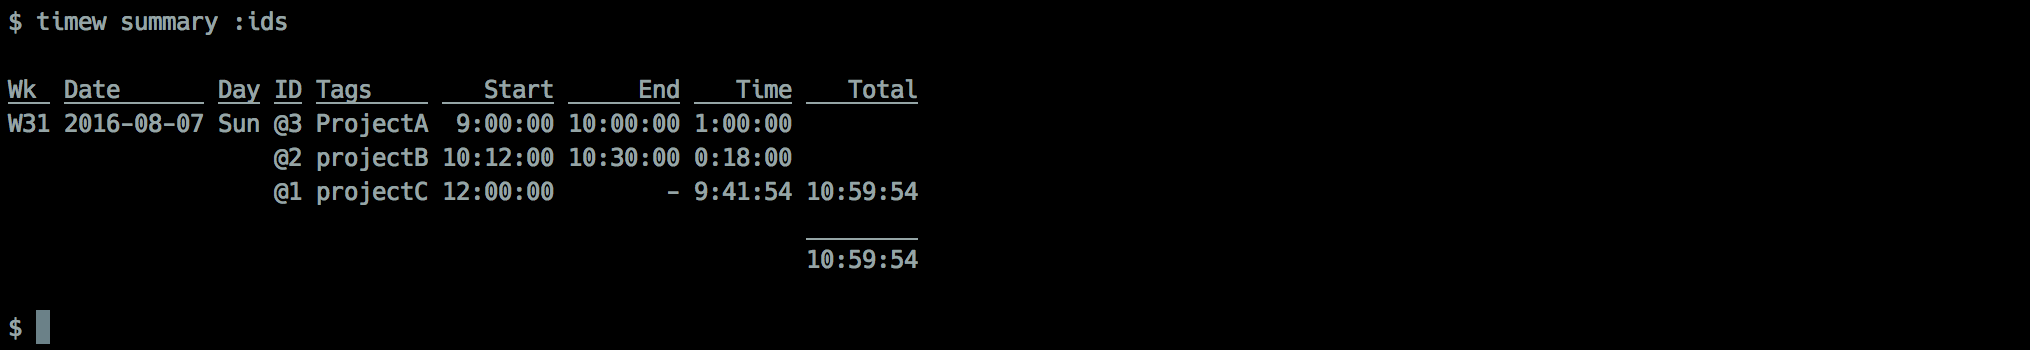
\includegraphics[width=12cm]{images/tutorial38.png}
\end{frame}

\begin{frame}[fragile]\frametitle{Corrections (3)}
    Notice how the intervals now have IDs: \verb=@3= for the oldest interval. Let's make some corrections:

    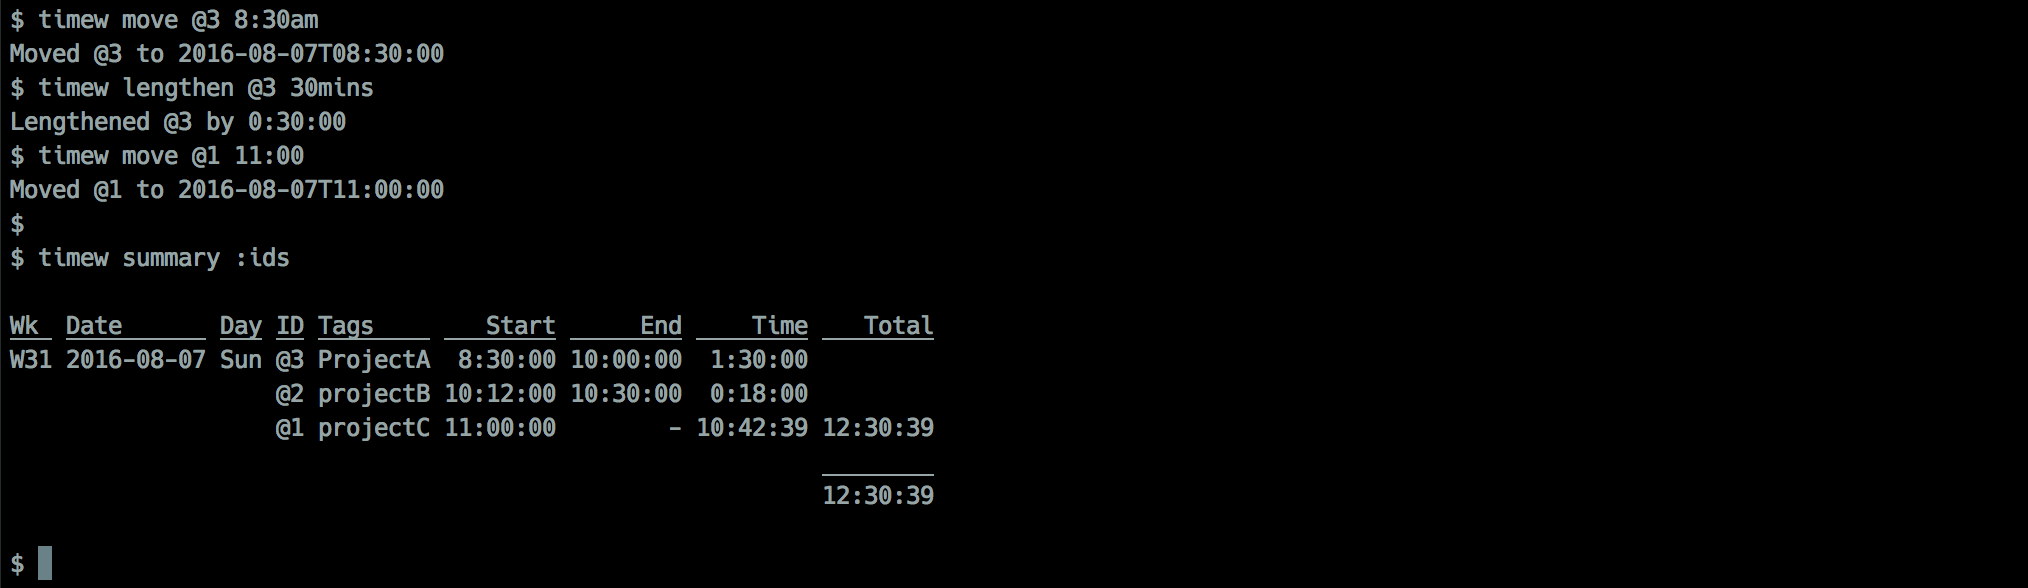
\includegraphics[width=12cm]{images/tutorial39.png}
\end{frame}

\begin{frame}[fragile]\frametitle{Corrections (4)}
    There is still a problem, interval \verb=@2= needs to occupy the slot between 10am and 11am. There is a \verb=:fill= hint that does this for us.

    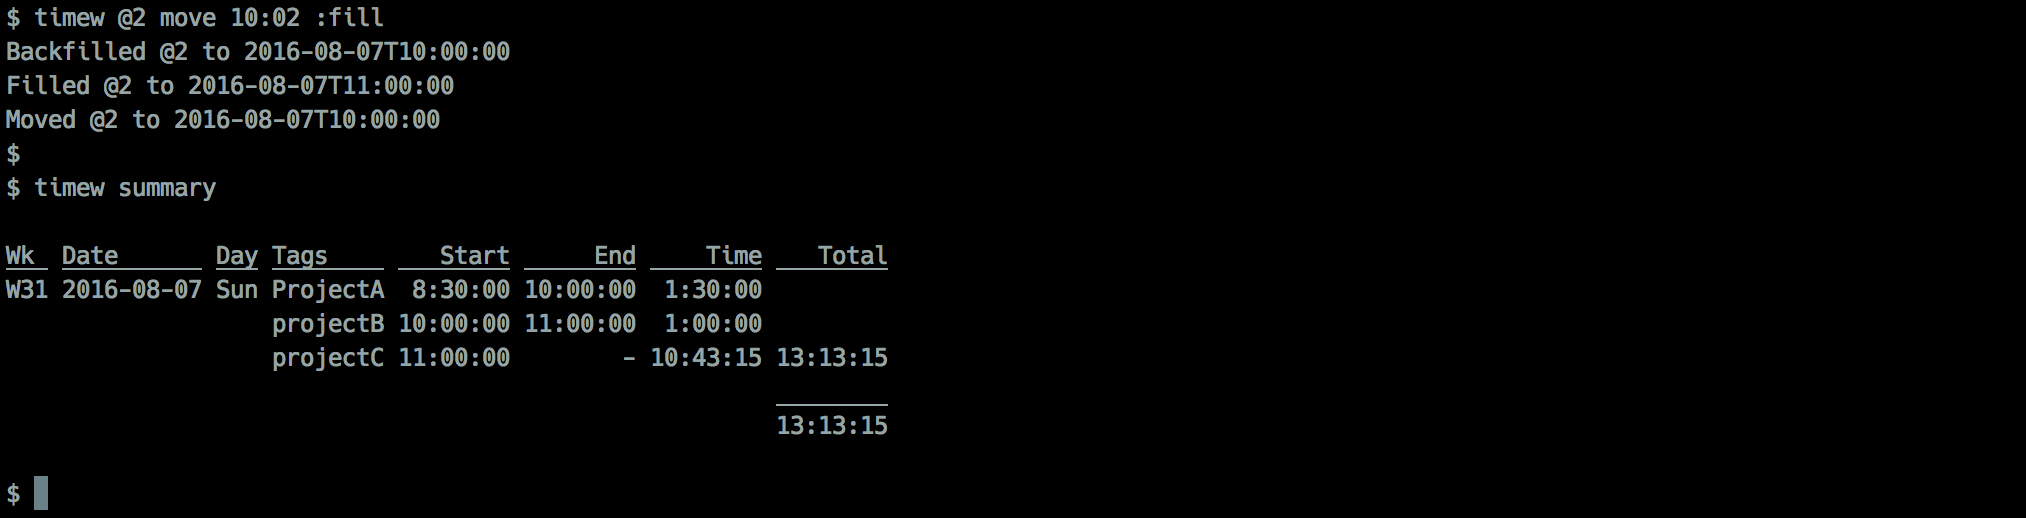
\includegraphics[width=12cm]{images/tutorial40.png}

    The \verb=@1= ID always represents the newest interval. Note that if my corrections have changes the order, then the IDs would be different, and you would need to run \verb=timew summary :ids= again to see the new IDs.
\end{frame}

\begin{frame}[fragile]\frametitle{Corrections (5)}
    Finally, I actually stopped for lunch at 12:30 for 45 minutes:

    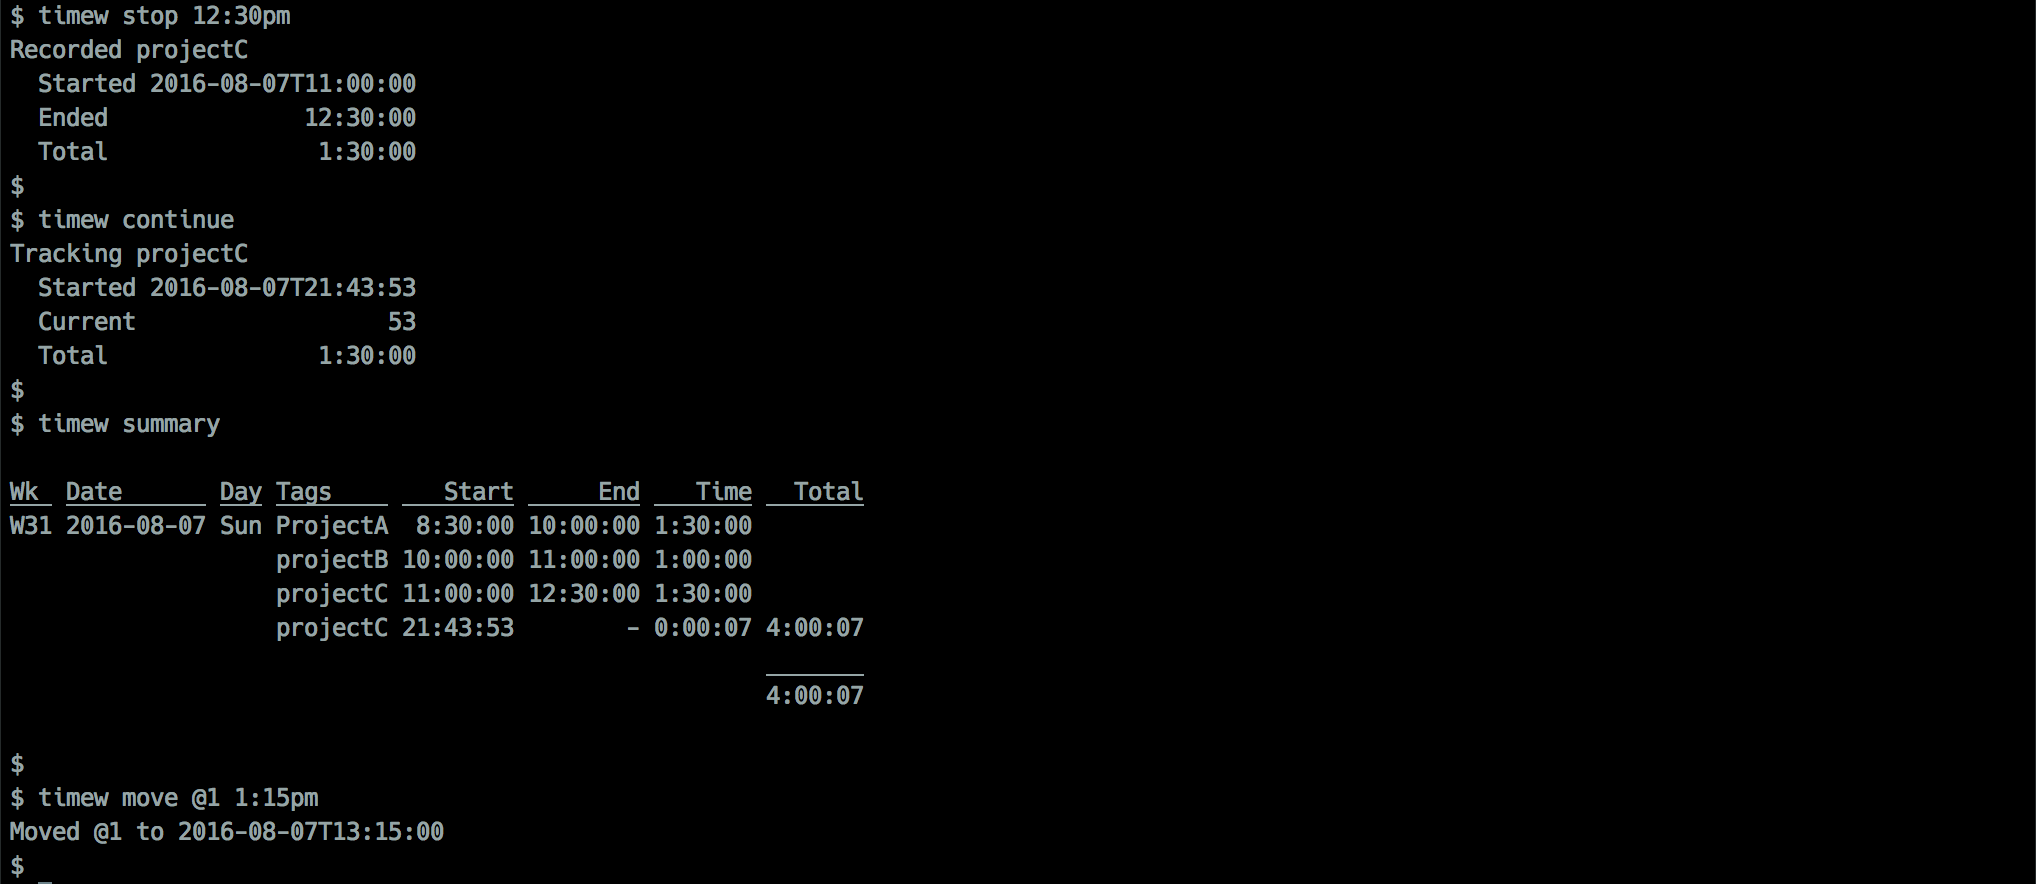
\includegraphics[width=12cm]{images/tutorial41.png}
\end{frame}

\begin{frame}[fragile]\frametitle{Corrections (6)}
    Let's keep going, even though this example has already exceeded credibility, to demonstrate more. I need to change that \textit{projectB} interval to use \textit{projectB1} and \textit{projectB2} tags, and divide the time between the two. We will split the interval, the re-tag it.

    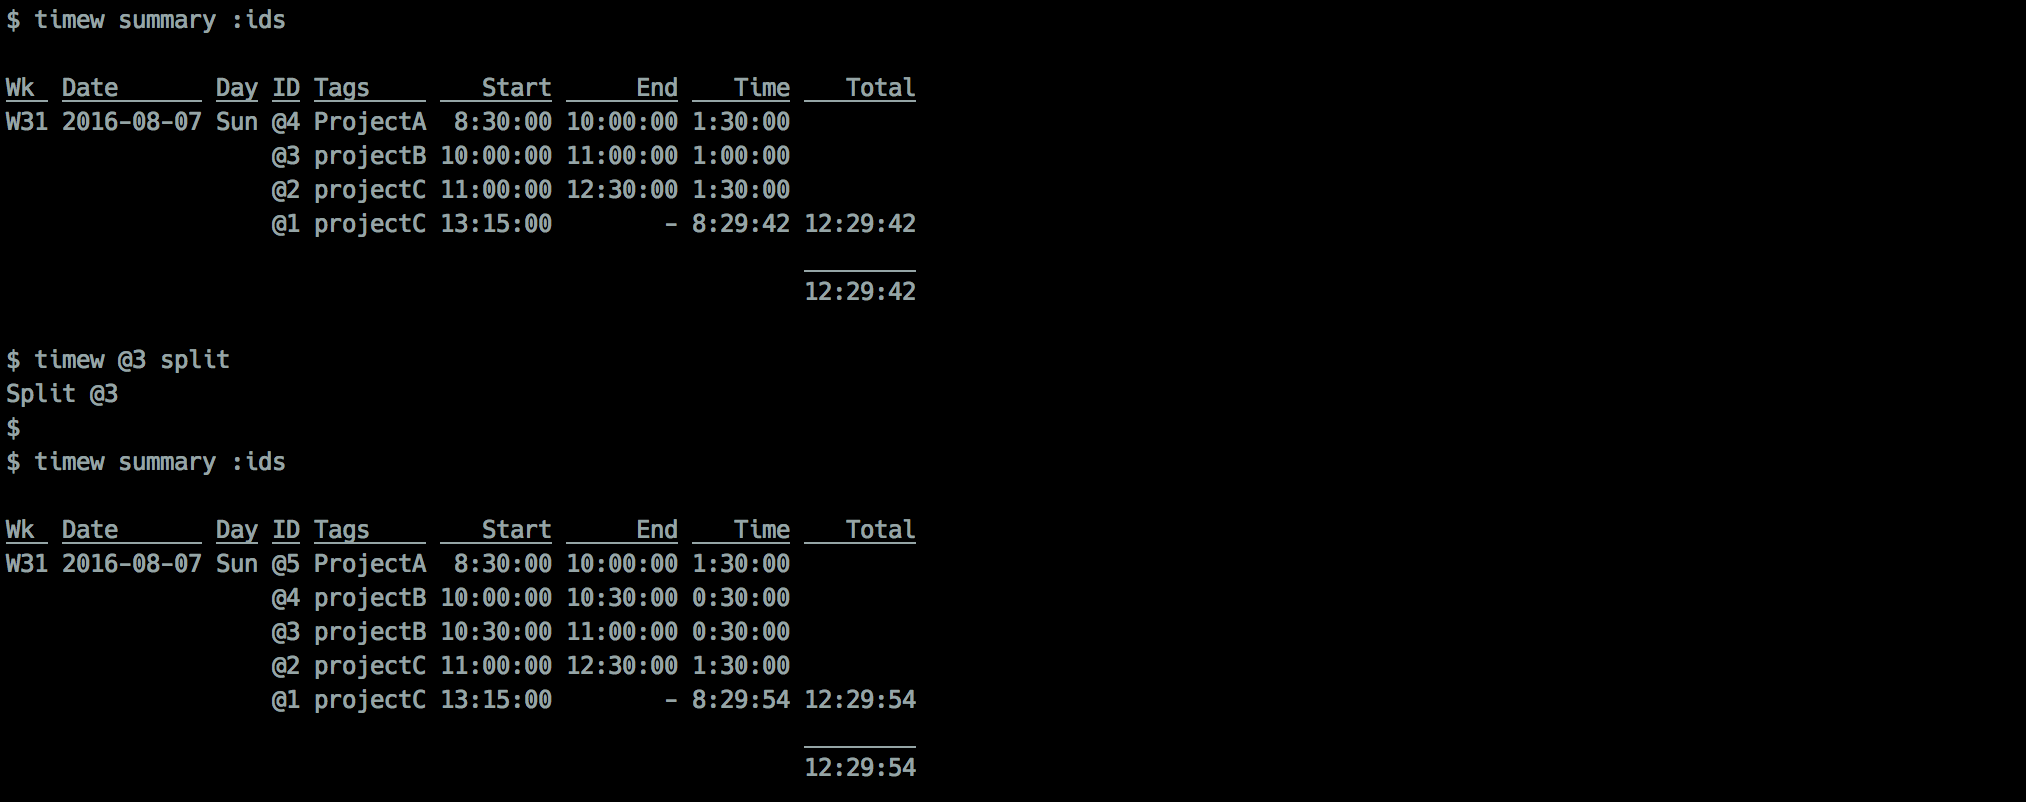
\includegraphics[width=12cm]{images/tutorial42a.png}
\end{frame}

\begin{frame}[fragile]\frametitle{Corrections (7)}
    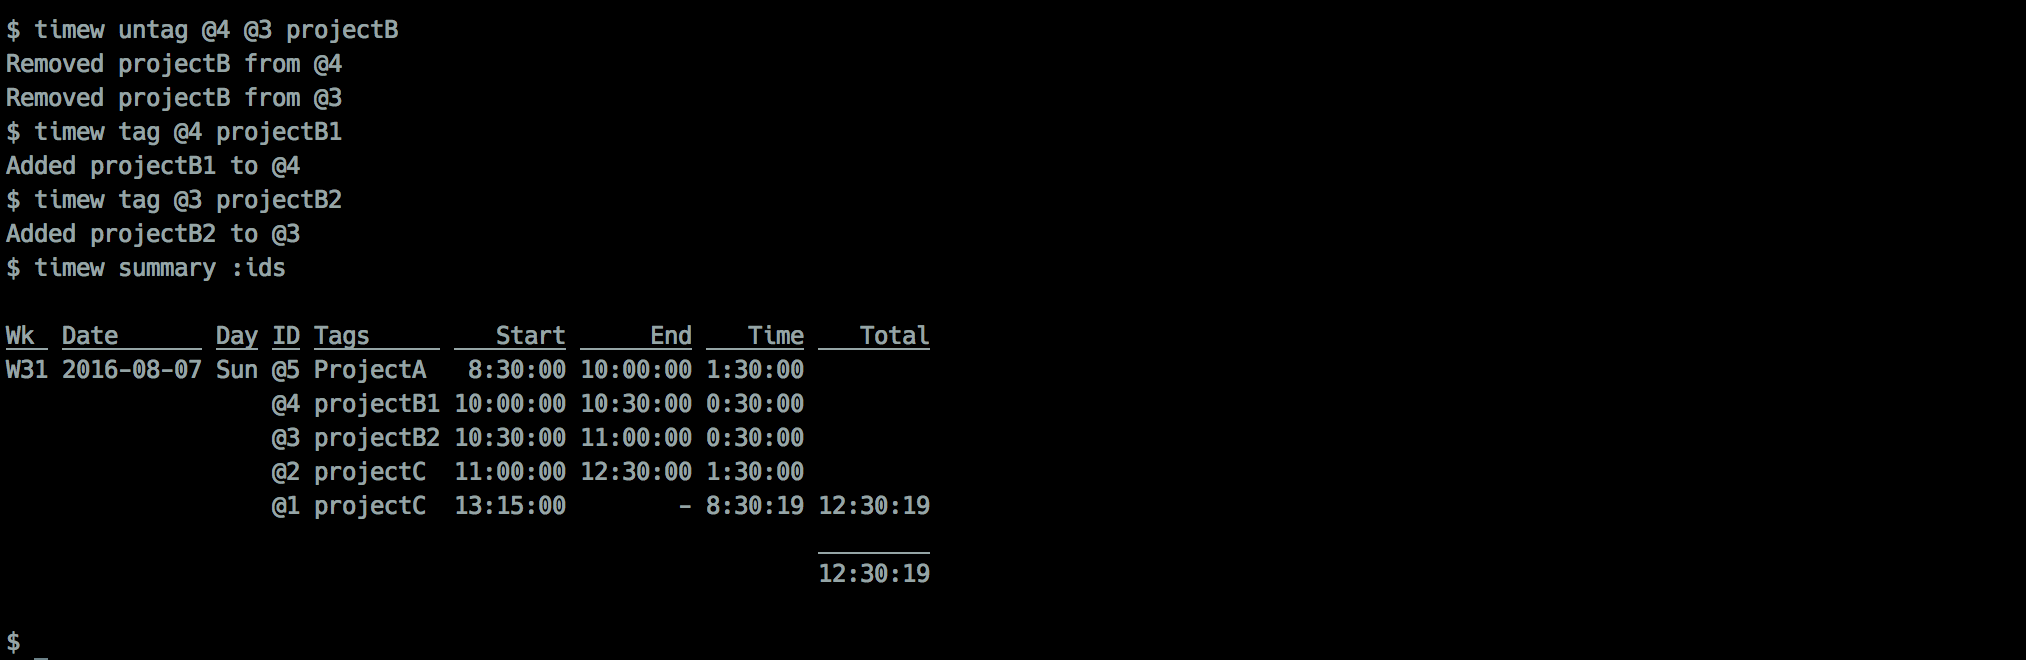
\includegraphics[width=12cm]{images/tutorial42b.png}

    Notice how the \verb=split= command just divided \verb=@3= into two even-sized intervals. But we're still not done - I brought lunch to work and ate at my desk while working so let's eliminate that lunch break.
\end{frame}

\begin{frame}[fragile]\frametitle{Corrections (8)}
    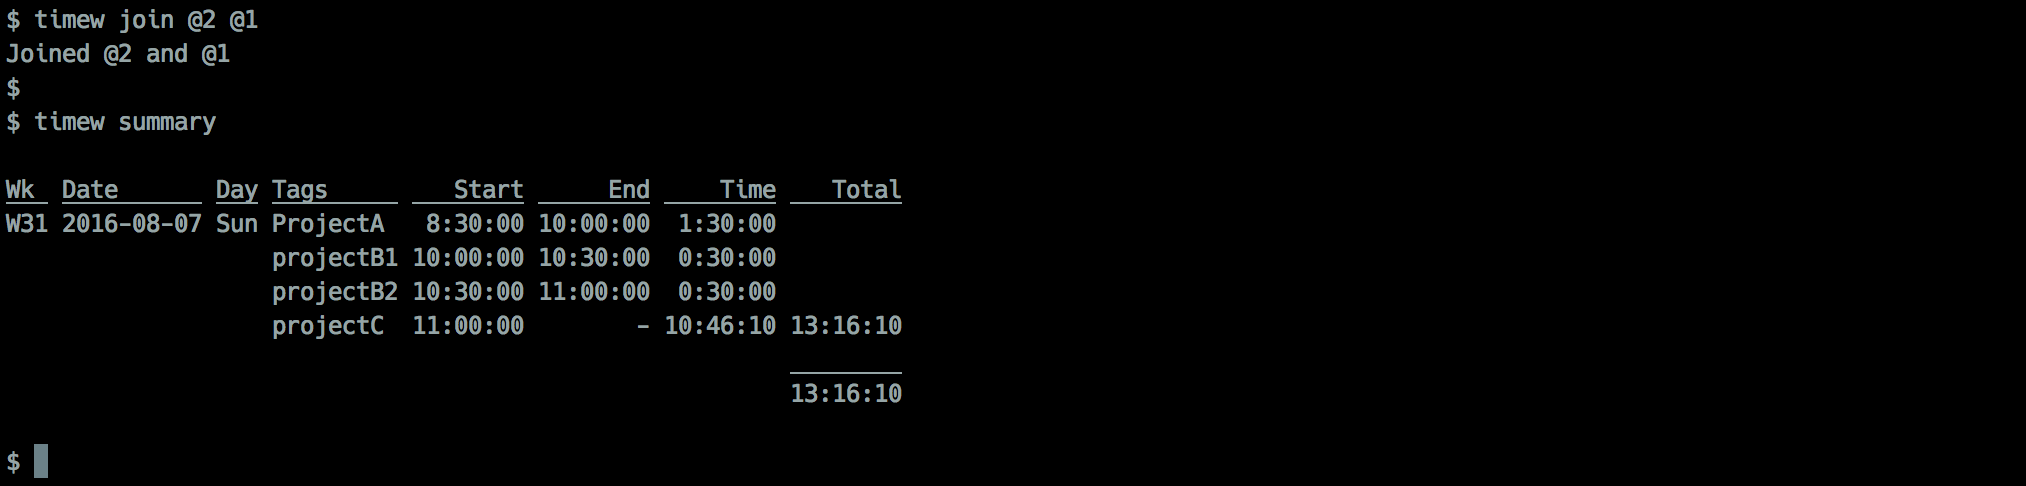
\includegraphics[width=12cm]{images/tutorial43.png}

    Now whether this report now accurately represents your day, or whether it is a fiction you need to report (no judgement here), Timewarrior supports it, but let's stop - the example can't take much more.

    We saw the \verb=stop= command with a specific end time, the \verb=move=, the \verb=lengthen=, \verb=split=, \verb=join=, \verb=tag= and \verb=untag= commands and the \verb=:fill= hint being used. There are also the \verb=shorten=, \verb=cancel=, and \verb=delete= commands.  See \verb=man timew= for full details.
\end{frame}

\begin{frame}[fragile]\frametitle{Extensions}
    Timewarrior reports are not sophisticated, they are minimally functional and focus on simply displaying the data. What if you need a report broken down by tags, with weekly subtotals?

    Timewarrior supports extension reports, via the \href{https://taskwarrior.orgdocs/timewarrior/api.html}{extension API}. This is mechanism that allows you to write a report using any language you choose. Don't like the way the summary report shows the data? Write your own. Better yet, share the result, and we'll build a list of 3rd party reports.

    We've included one extension report with Timewarrior, and will add more. The one provided is:

    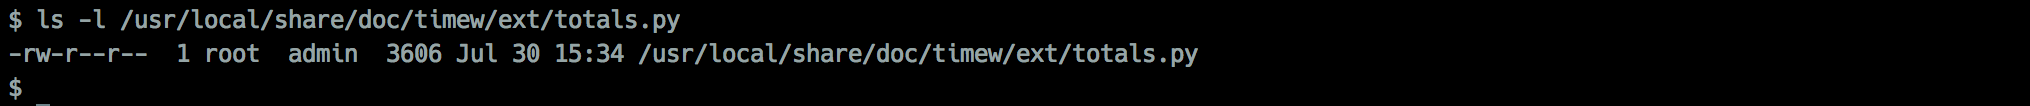
\includegraphics[width=12cm]{images/tutorial44.png}

    Again, that path is platform-dependent, so use the appropriate path for your system.
\end{frame}

\begin{frame}[fragile]\frametitle{Extensions (2)}
    Note that this is a Python script, and to use this you'll need to have Python installed.

    To install and use this extension, or any other, simply copy it to your \verb=~/.timewarrior/extensions= directory and make sure it is executable.

    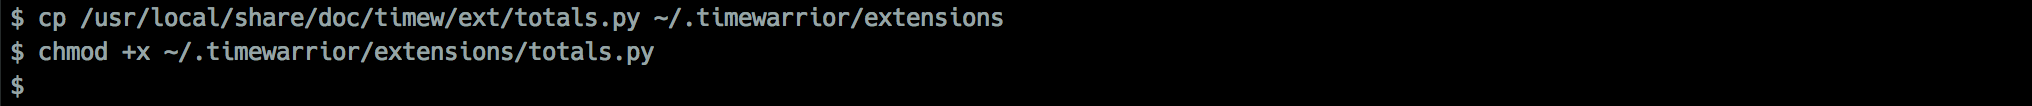
\includegraphics[width=12cm]{images/tutorial45.png}
\end{frame}

\begin{frame}[fragile]\frametitle{Caution}
    \textbf{Extensions are dangerous things}.

    As with any downloaded program, be careful -- you are giving execute permission to software that may harm you.

    Fortunately this is the world of open source, and while that does not mean the software is safe, it does mean you have the necessary access to audit the code and prove it is safe.

    If you find the code safe, use it. If you are unsure, don't.

    Once the extension is in the \verb=extensions= directory, and executable, it should be visible to the \verb=extensions= command.

    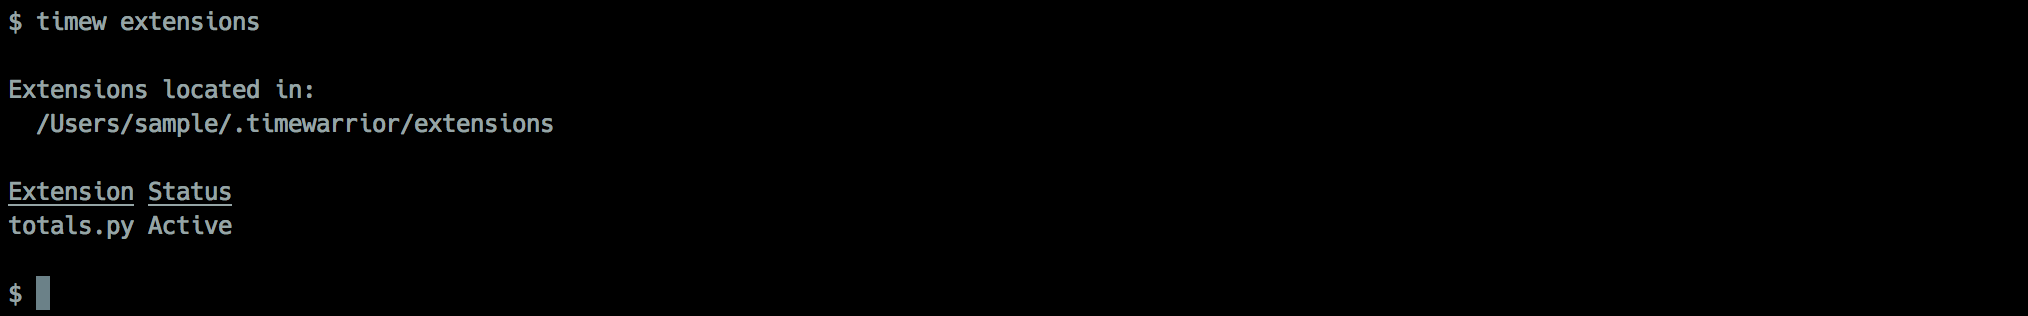
\includegraphics[width=12cm]{images/tutorial46.png}
\end{frame}

\begin{frame}[fragile]\frametitle{Caution (2)}
    Additionally, the \verb=diagnostics= command will report the presence and status of this extension.

    Once an extension is ready to use, it is used in the same way that the \verb=summary= report is used, with date range and/or tag filtering. The command you use is compared to the name of the script, and if unique, is a match. All of these commands are equivalent:

    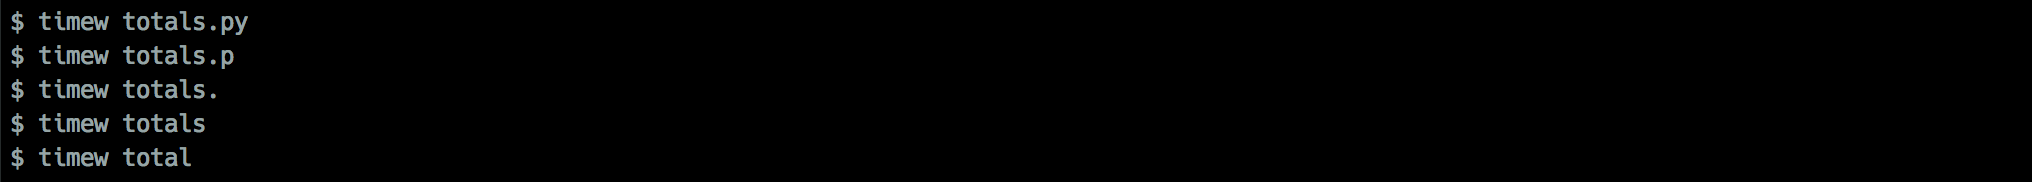
\includegraphics[width=12cm]{images/tutorial47.png}
\end{frame}

\begin{frame}[fragile]\frametitle{Caution (3)}
    Here is the report run with no filter, and therefore against all recorded data, which is not much in this example.

    \includegraphics[width=12cm]{images/tutorial48.png}

    Extensions are not restricted to emitting text, they could for example output HTML, DOT, PDF, PNG, JPEG \ldots
\end{frame}

\section{Integration in Takswarrior}

\begin{frame}[fragile]\frametitle{Integration}
    Timewarrior integrates with Taskwarrior by means of a Taskwarrior \verb=on-modify= hook script. Once installed, this means that whenever a task is active, Timewarrior is used to track the time.

    To install the script, copy it into your Taskwarrior directory:

    \includegraphics[width=12cm]{images/tutorial49.png}

    Again, that path is platform-dependent, so use the appropriate path for your system.
\end{frame}

\begin{frame}[fragile]\frametitle{Integration (2)}
    Now we can create a task, start it, complete it and automatically track it.

    \includegraphics[width=12cm]{images/tutorial50.png}

    The \verb=on-modify.timewarrior= hook script captures the task description and all tags and passes these to Timewarrior as tags. If a project was assigned (it was not in this example) then it too would have been passed as a tag.

    Is this behavior modifiable?  Yes, this is open source, and the hook script is written in Python.
\end{frame}

\begin{frame}[fragile]\frametitle{Links}
    This talk was shamelessly converted from the \href{https://taskwarrior.org/docs/timewarrior/tutorial.html}{Online Tutorial}, there are more detailed \href{https://taskwarrior.orgdocs/timewarrior/index.html}{Online Docs}.

    Starting today, there is XXX as well.

    Feedback is highly appreciated!
\end{frame}

\end{document}
